%%% Result --- 
%% 
%% Filename: result.tex
%% Author: Jacob Ringfjord & Max Wilén
%%% Code:

\chapter{Result}
\label{cha:result}

The Result chapter is structured into two main sections. The first section provides an overview of the developed tool, highlighting its features and functionality. The second section presents an analysis of the tool's performance.

\section{Pipeline Analysis Report}
\label{sec:result:pipeline_analysis_report}


\begin{figure}
    \centering
    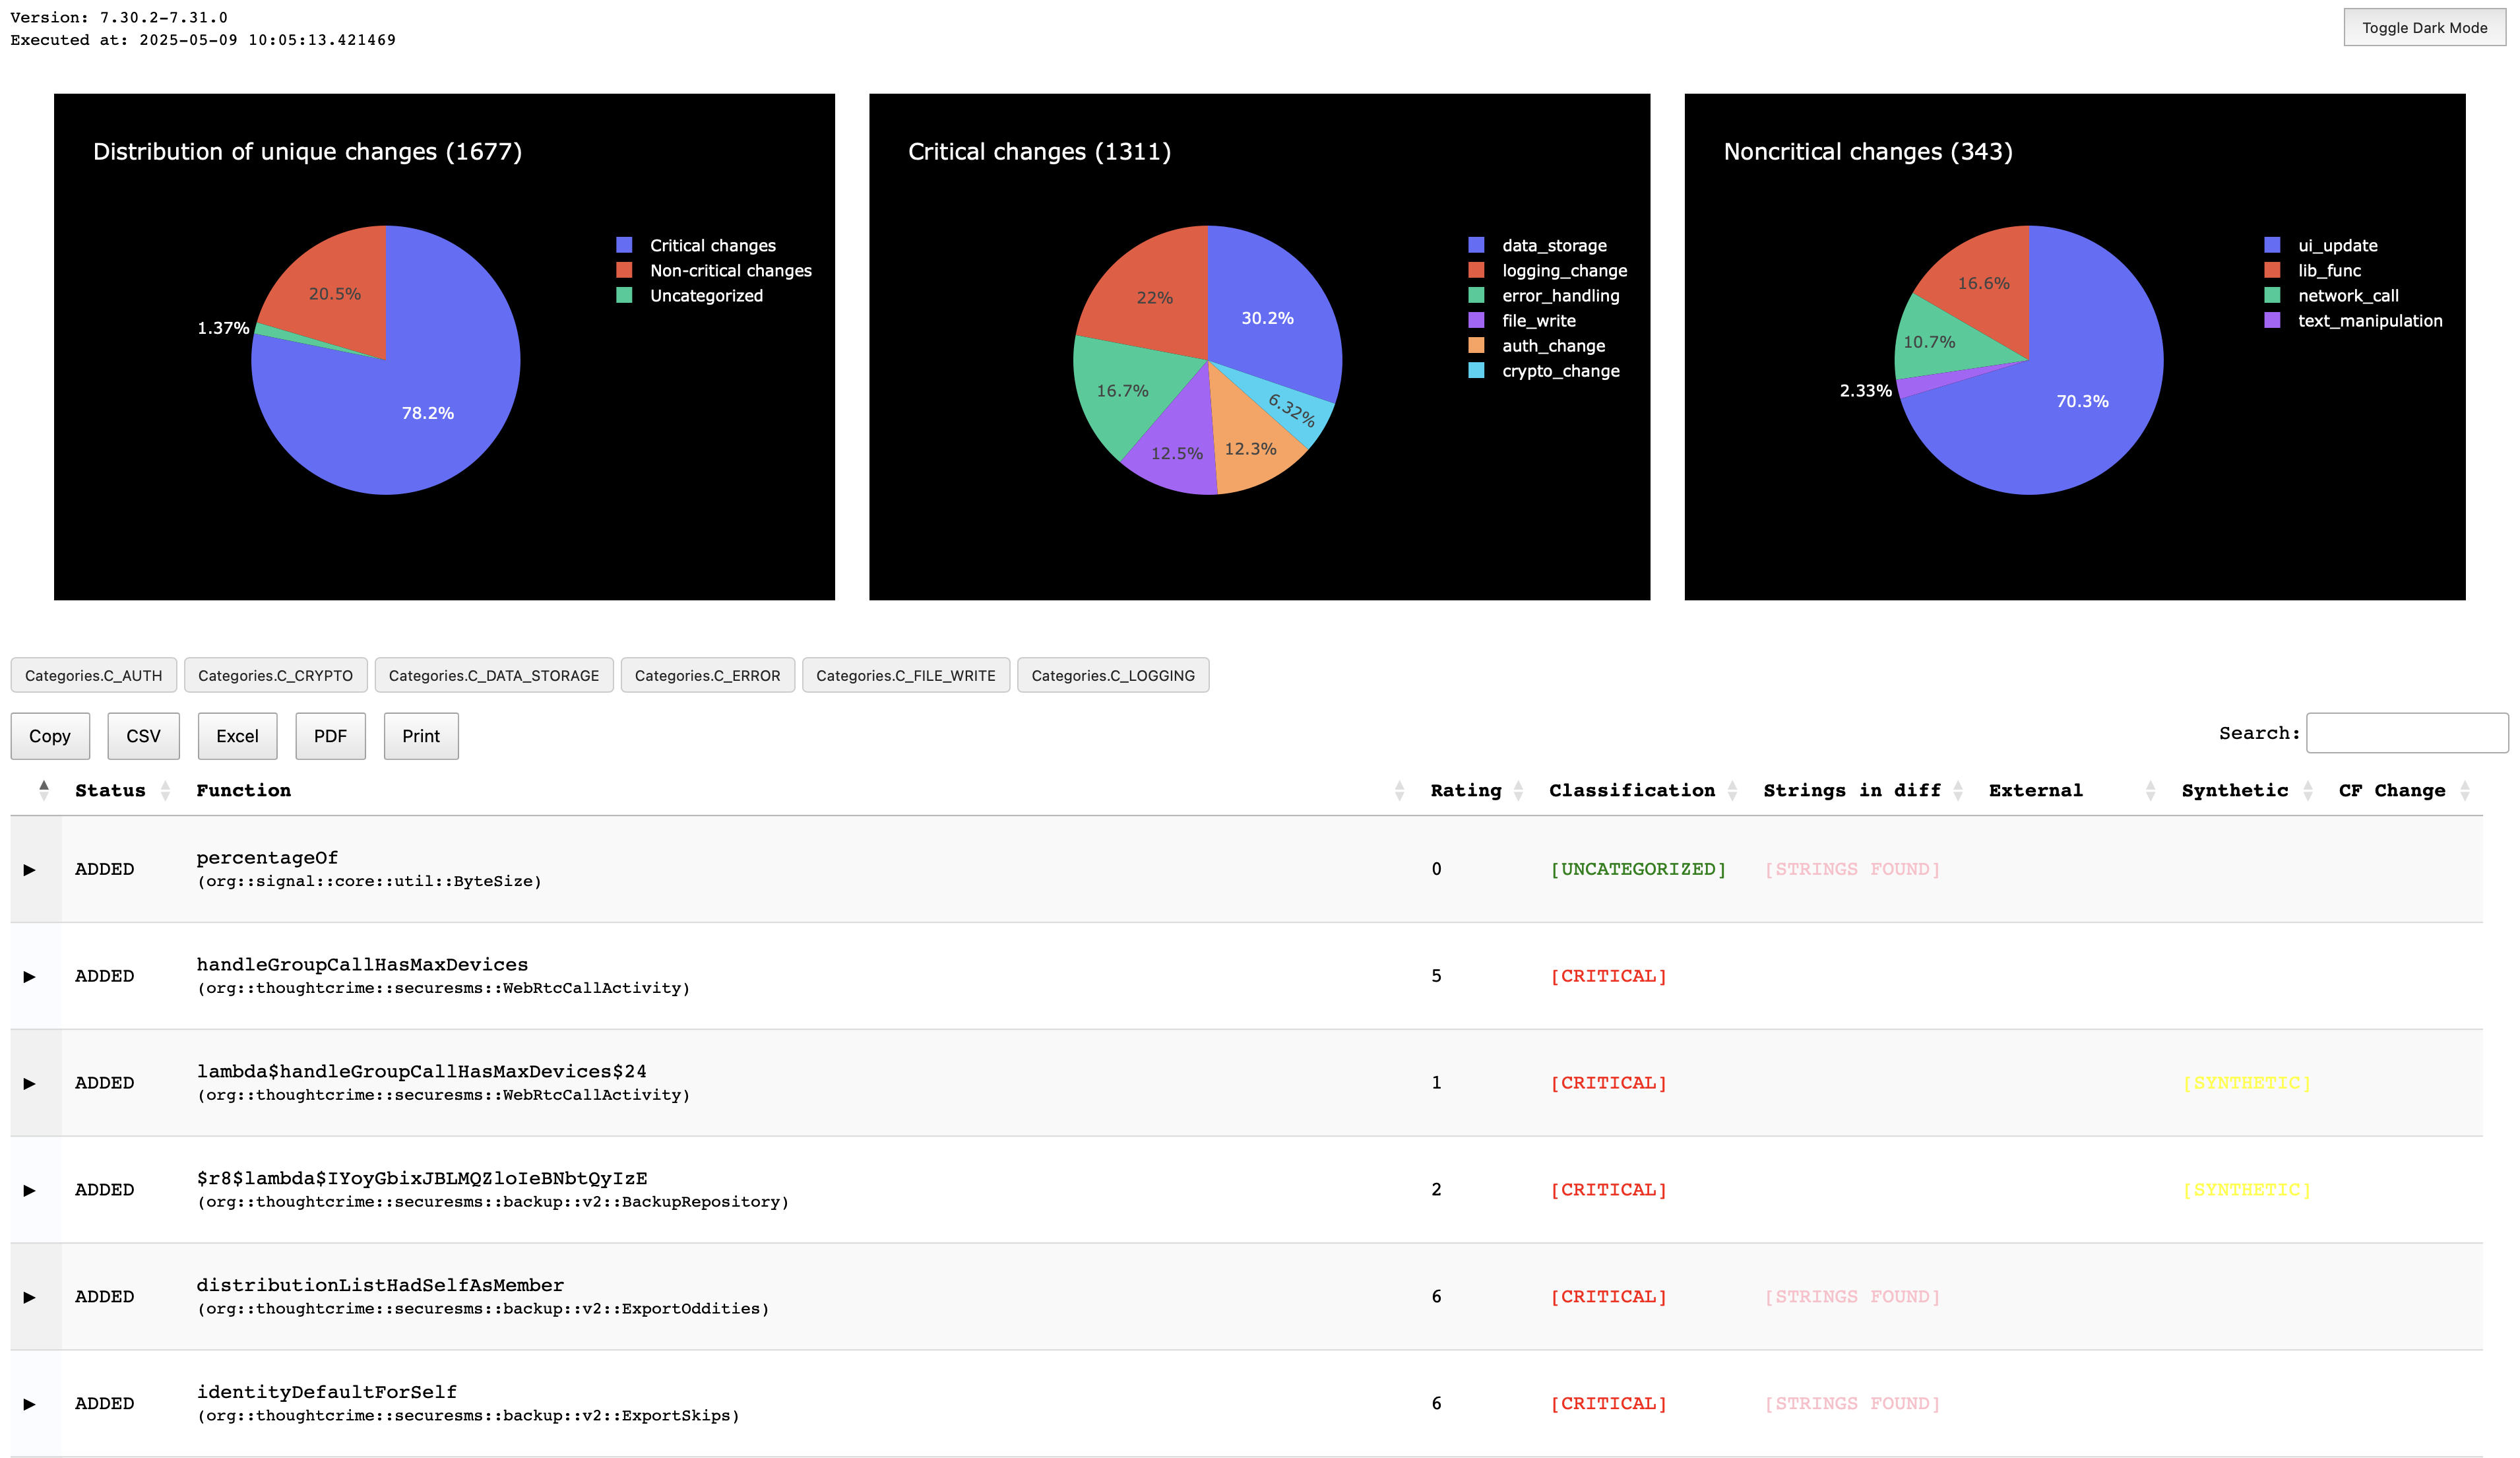
\includegraphics[width=1\linewidth]{figures/results/report_screenshots/report_front_page.png}
    \caption{Screenshot of the HTML report front page}
    \label{fig:pipeline_frontpage}
\end{figure}

\begin{figure}
    \centering
    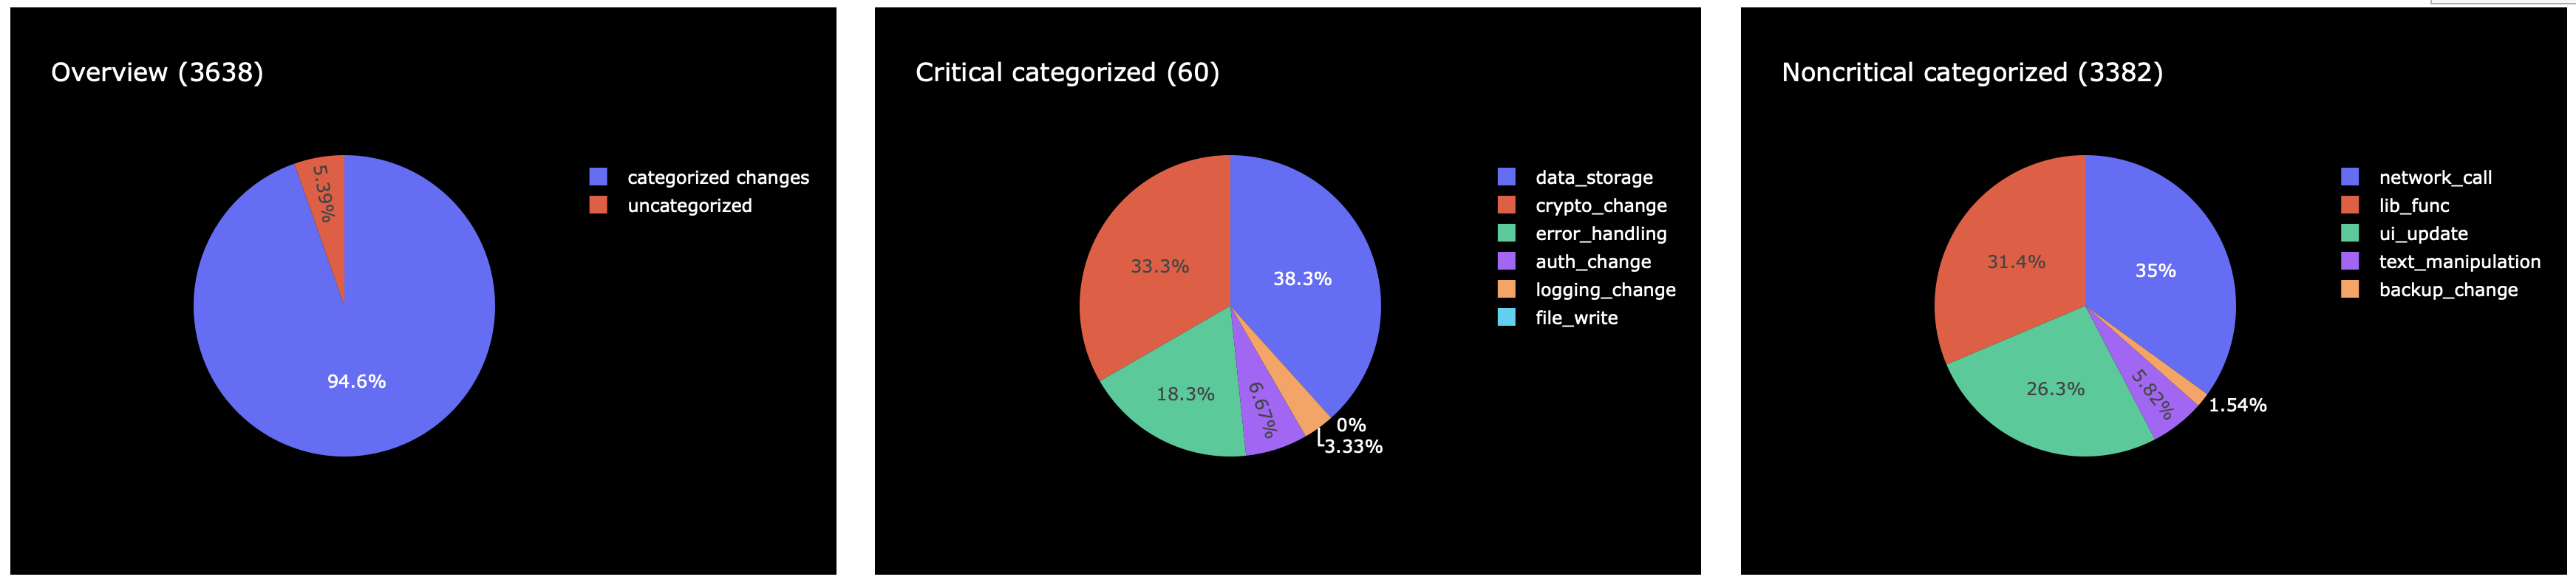
\includegraphics[width=1\linewidth]{figures/results/report_screenshots/diagrams.png}
    \caption{Screenshot of the pie charts showing the categorization and classification distributions}
    \label{fig:pipeline_piecharts}
\end{figure}

This section presents the HTML report generated by the tool after its analysis. The generated report provides a detailed view of the analysis results, including key features and layout elements. Each feature is explained in a dedicated subsection, describing its functionality. The data in the figures is purely illustrative and should be regarded as an example of the report's format and content.

Figure \ref{fig:pipeline_frontpage} illustrates the full-width front page of the HTML report. At the top of this report, three pie charts provide a visual summary of the categorization results generated by the pipeline. A more focused view of these pie charts is presented in Figure \ref{fig:pipeline_piecharts}, offering a closer look at the distribution of categorized changes.


Figure \ref{fig:pipeline_filtering_categories} presents the category filtering section of the HTML report. This section is designed to help users explore and analyze the changes detected in the analyzed software versions. Each button in this section represents a category identified by the pipeline during the analysis process.

\begin{comment}
These categories are used to classify the detected changes based on their nature and impact. They are broadly divided into two types: critical and non-critical categories. Critical categories include changes that directly affect the application's core functionality, security, or data handling. Examples of critical categories are data storage changes, which involve modifications in how data is read, written, or stored; authentication changes, which affect login mechanisms, session management, or token validation; cryptographic changes, which involve updates to encryption algorithms, key management, or hashing techniques; and file write changes, which relate to modifications in file-writing processes, such as creating, modifying, or deleting files.
\end{comment}

\begin{figure}
    \centering
    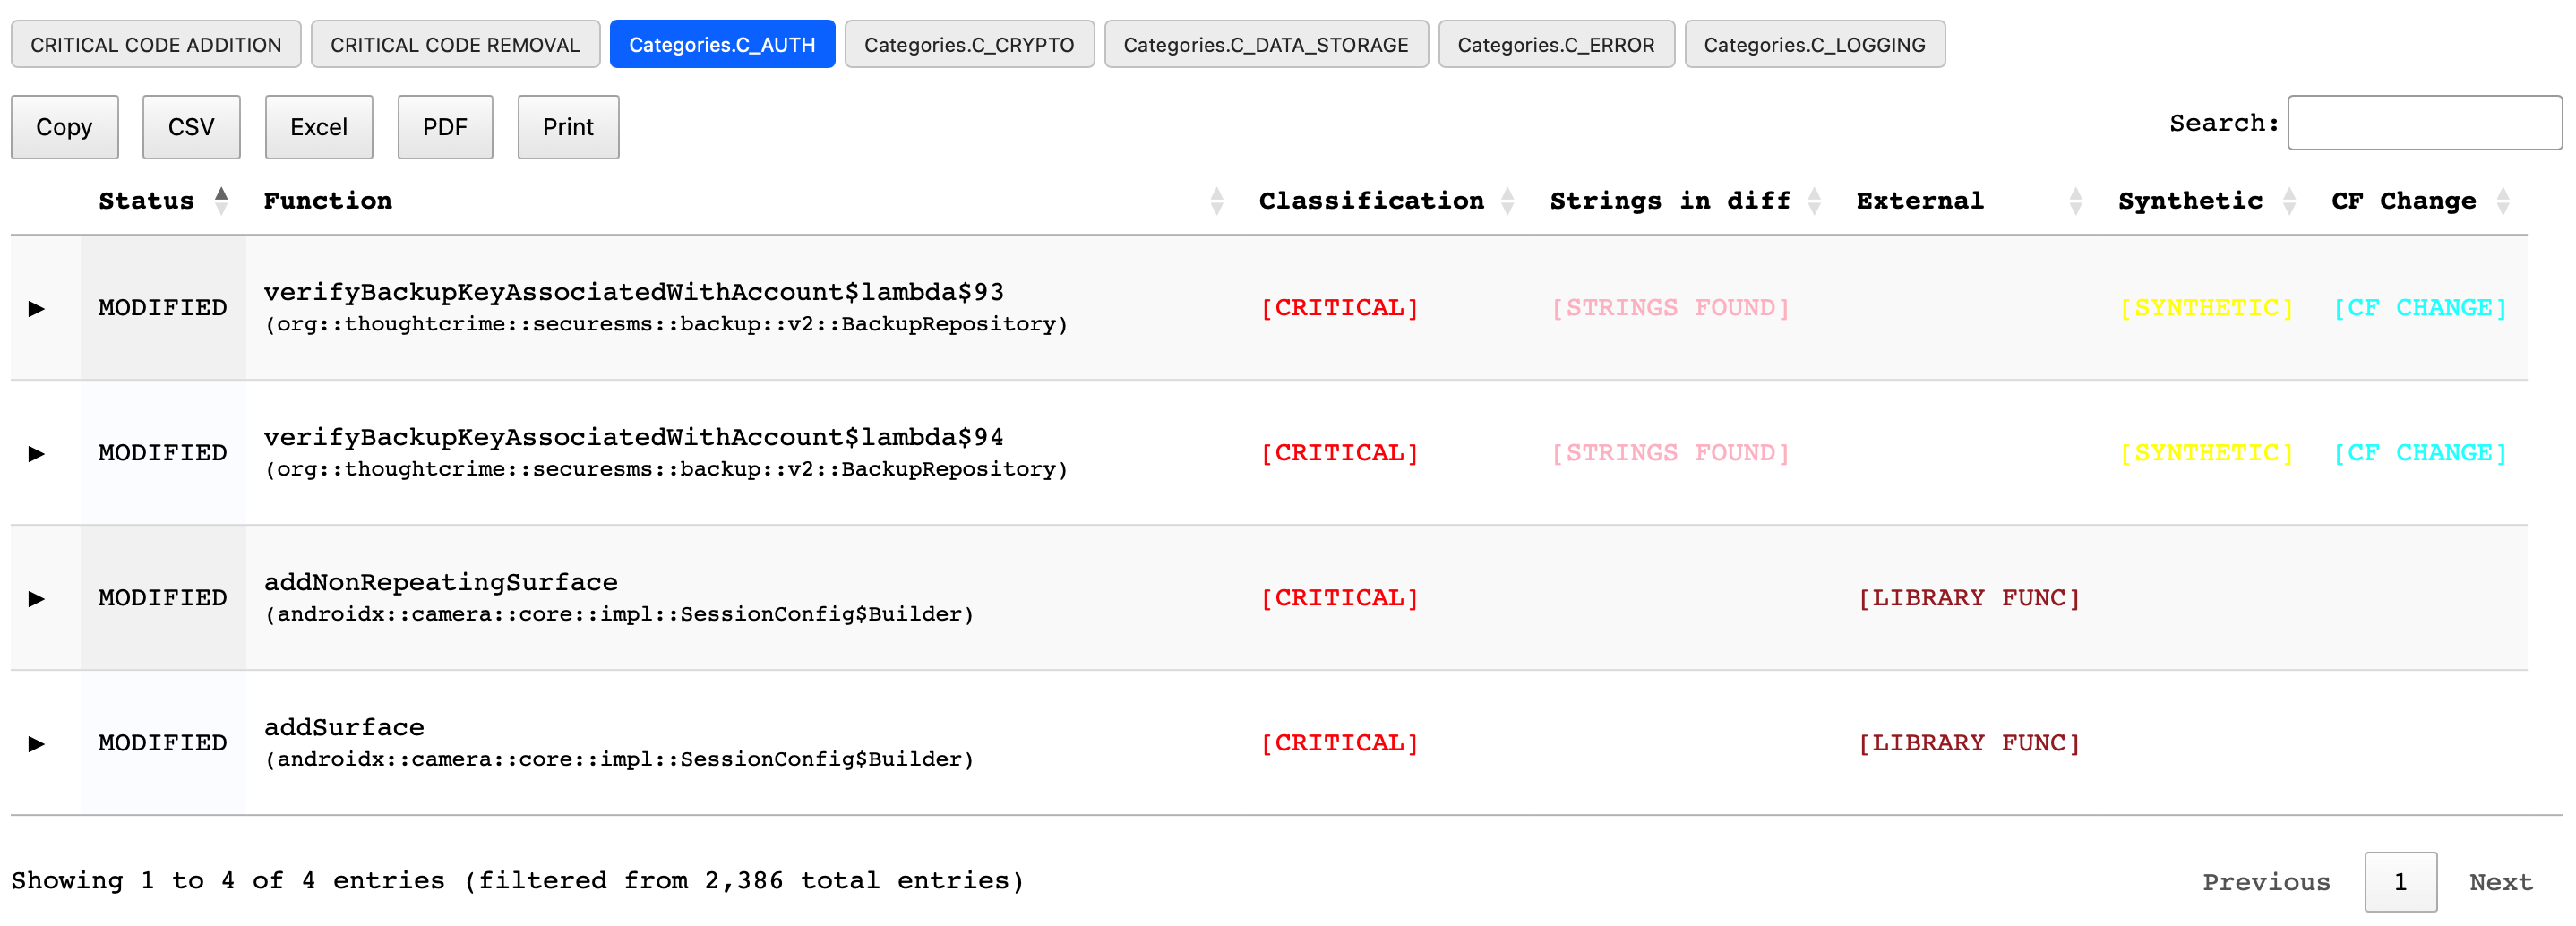
\includegraphics[width=1\linewidth]{figures/results/report_screenshots/feature_filtering.png}
    \caption{Filtering on changes which has been defined as Authentication handling}
    \label{fig:pipeline_filtering_categories}
\end{figure}

\begin{comment}
Non-critical categories, on the other hand, capture less impactful but still relevant changes, such as UI updates (alterations in user interface elements like layouts and colors), network calls (changes in API requests, endpoints, or response handling), and library functions (updates to external libraries or imported functions).
\end{comment}

By clicking on any of these category buttons, users can filter the displayed changes to focus only on those matching the selected category. Multiple categories can be selected simultaneously, with the filter combining them to provide a flexible and precise view of the categorized changes. This filtering system allows users to quickly identify and focus on the most relevant modifications, streamlining the analysis process.


Figure \ref{fig:pipeline_exporting} illustrates the export feature of the HTML report, positioned on the left side of the page. This section provides a set of buttons, each representing a different method for exporting the tabular data displayed in the report. Users can choose from various export formats, such as CSV, Excel, or PDF, allowing them to save the analyzed data for offline review or further analysis. It is important to note that this export functionality is limited to the data shown in the table and does not include the graphical diagrams or charts presented in the report. This separation ensures that users can efficiently export only the detailed, categorized results they are interested in.

\begin{figure}
    \centering
    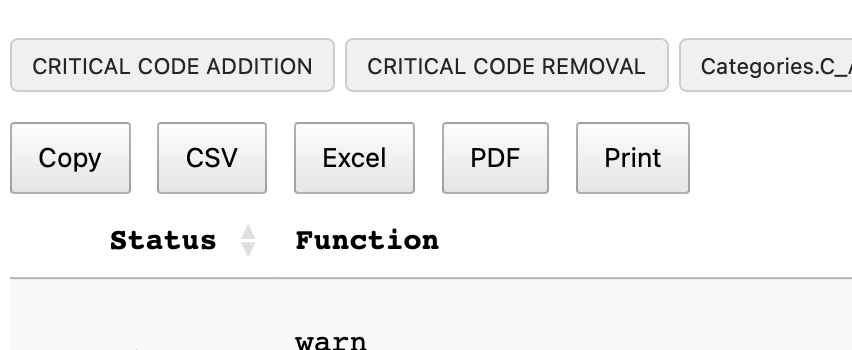
\includegraphics[width=0.5
    \linewidth]{figures/results/report_screenshots/feature_exporting.png}
    \caption{Exporting capabilities for data shown in tabular}
    \label{fig:pipeline_exporting}
\end{figure}

The HTML report provides a search field located next to the export buttons, making it easy for users to quickly find specific information. By entering a search term, users can filter the table, showing only the rows where the search term appears. For example, if you search for a function name or part of a file path, only rows matching that term will be displayed, while everything else is hidden. This feature, shown in Figure \ref{fig:pipeline_searchfield}, helps users focus on the most relevant data.

Just below the export buttons and the search field is the main data table. This table is organized in a simple row-and-column format, where each row represents a detected change, and each column shows details about that change, such as its category, function name, and other information. 

\begin{comment}
The layout makes it easy to review and understand the results and is presented in Figure \ref{fig:pipeline_datatable}.
\end{comment}

\begin{figure}
    \centering
    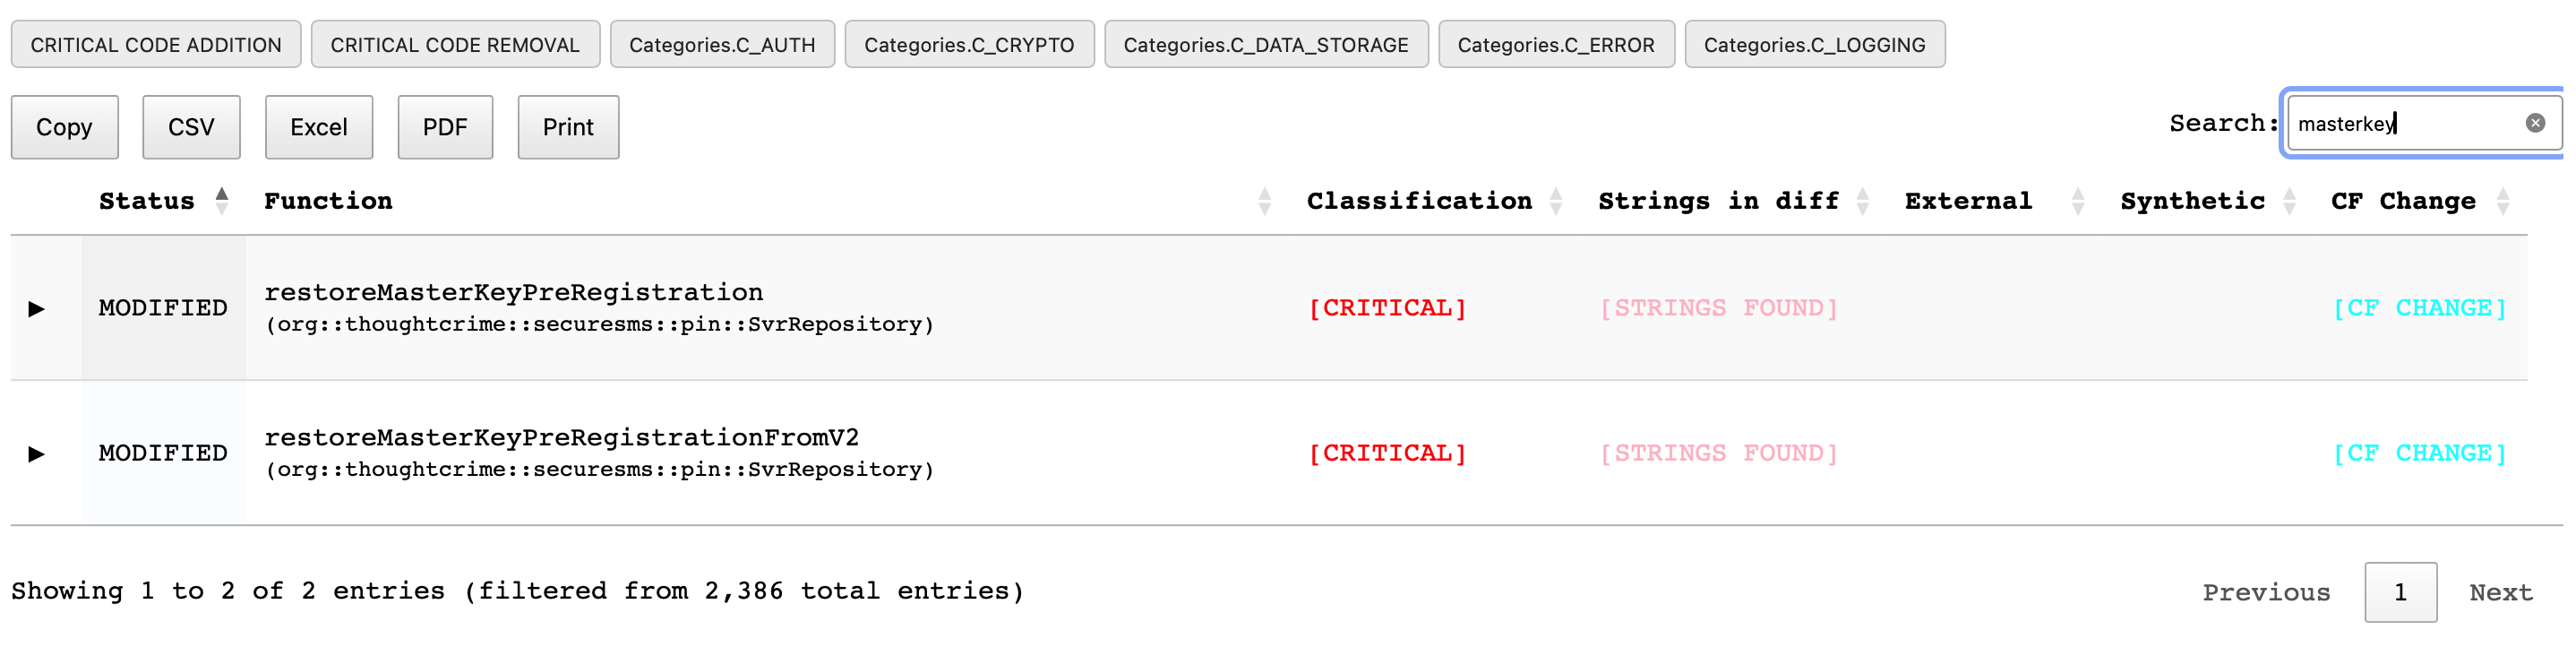
\includegraphics[width=1\linewidth]{figures/results/report_screenshots/feature_search.png}
    \caption{Searching for 'masterkey', which looks at the value of the \textit{Function} column}
    \label{fig:pipeline_searchfield}
\end{figure}



\begin{comment}
\begin{figure}
    \centering
    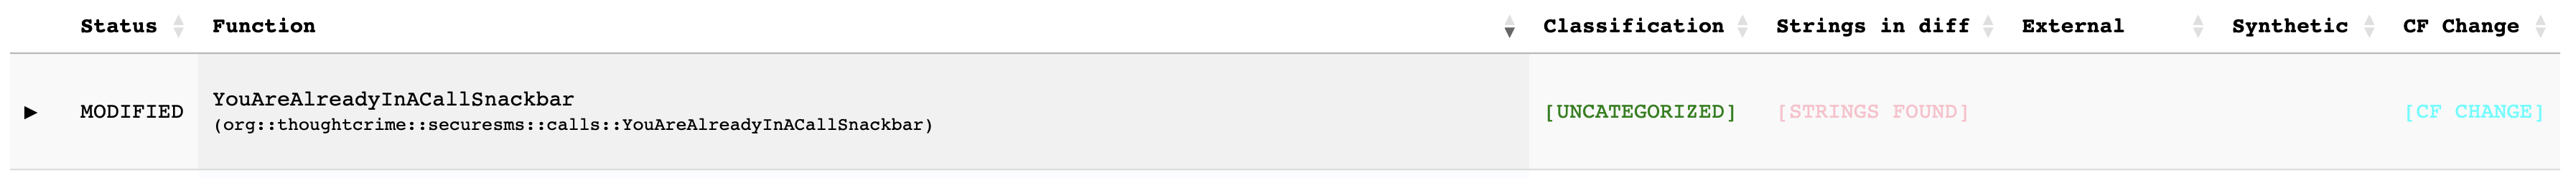
\includegraphics[width=1\linewidth]{figures/results/report_screenshots/table_columns.png}
    \caption{Caption}
    \label{fig:pipeline_datatable}
\end{figure}
\end{comment}


\begin{figure}
    \centering
    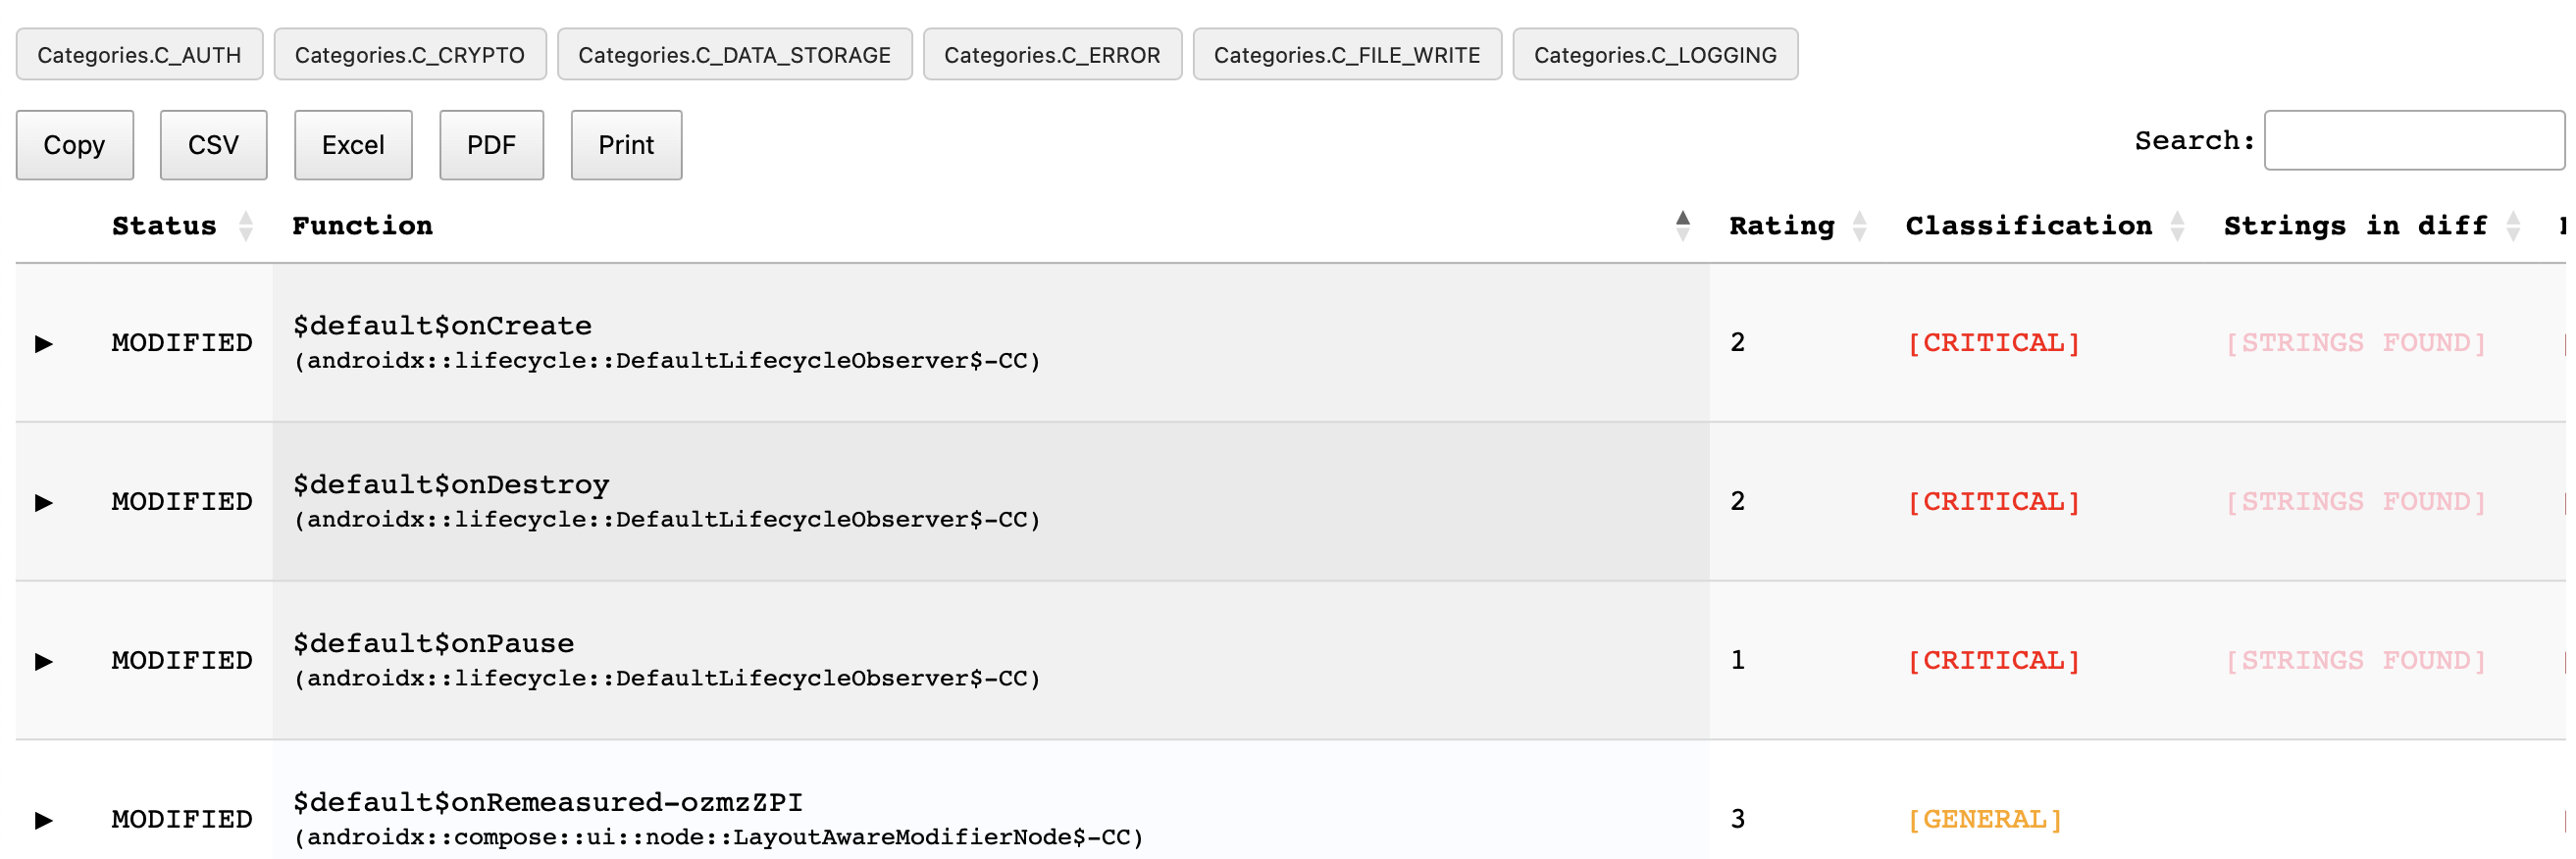
\includegraphics[width=1\linewidth]{figures/results/report_screenshots/feature_sorting1.png}
    \caption{Sorting on \textit{Classification} and \textit{Strings in diff}}
    \label{fig:pipeline_sorting_1}
\end{figure}

\begin{figure}
    \centering
    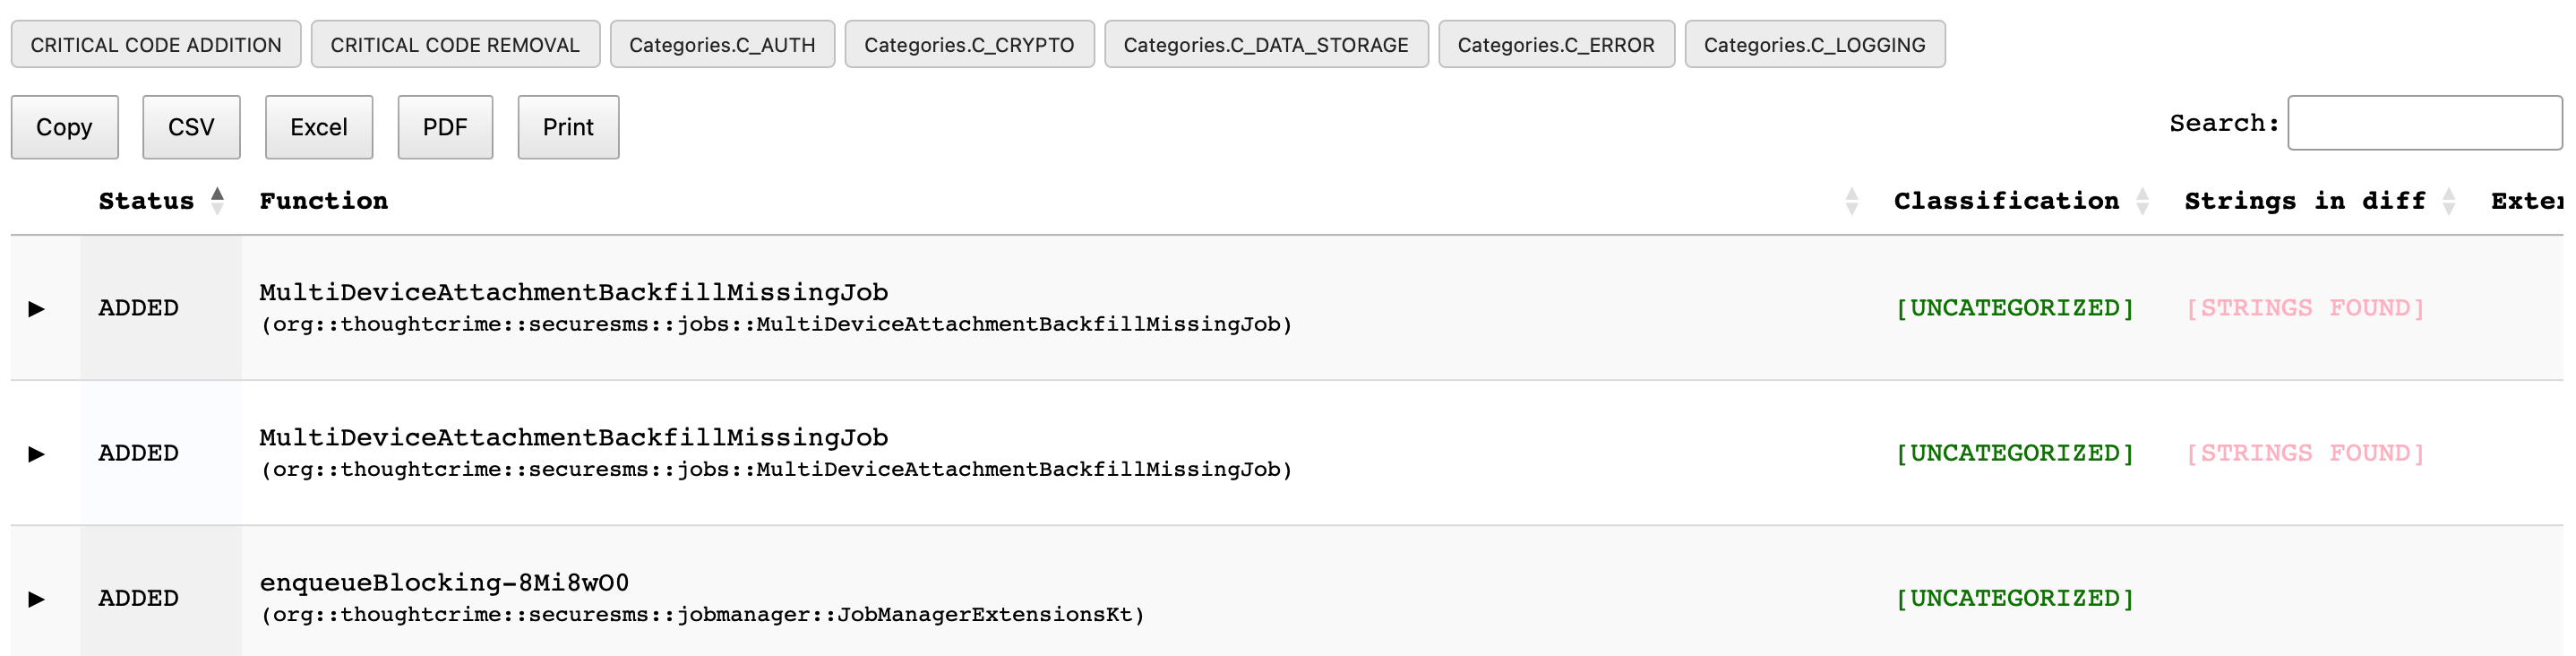
\includegraphics[width=1\linewidth]{figures/results/report_screenshots/feature_sorting2.png}
    \caption{Sorting on \textit{Function status} and \textit{Classification}}
    \label{fig:pipeline_sorting_2}
\end{figure}

The HTML report’s data table offers flexible sorting and detailed viewing options, making it easier for users to explore and analyze the detected changes. Users can sort the table by clicking on any column name, which immediately rearranges the rows based on the values in that column. For example, clicking on the Category column will sort the entries alphabetically by category. Moreover, the report supports multi-level sorting—users can achieve this by clicking multiple column names in sequence, allowing for more precise data organization. This functionality is illustrated in Figures \ref{fig:pipeline_sorting_1} and \ref{fig:pipeline_sorting_2}, which show two different sorting configurations.

Beyond sorting, the table provides an expandable row feature for in-depth analysis. Each row can be expanded to display additional information about the corresponding change, offering insights beyond the basic data shown in the main table. This detailed view reveals extra data collected during the change detection and categorization process, helping users better understand the nature of each modification. Figures \ref{fig:pipeline_detailedview1} and \ref{fig:pipeline_detailedview2} provide visual examples of how this expanded information is presented.

\begin{figure}
    \centering
    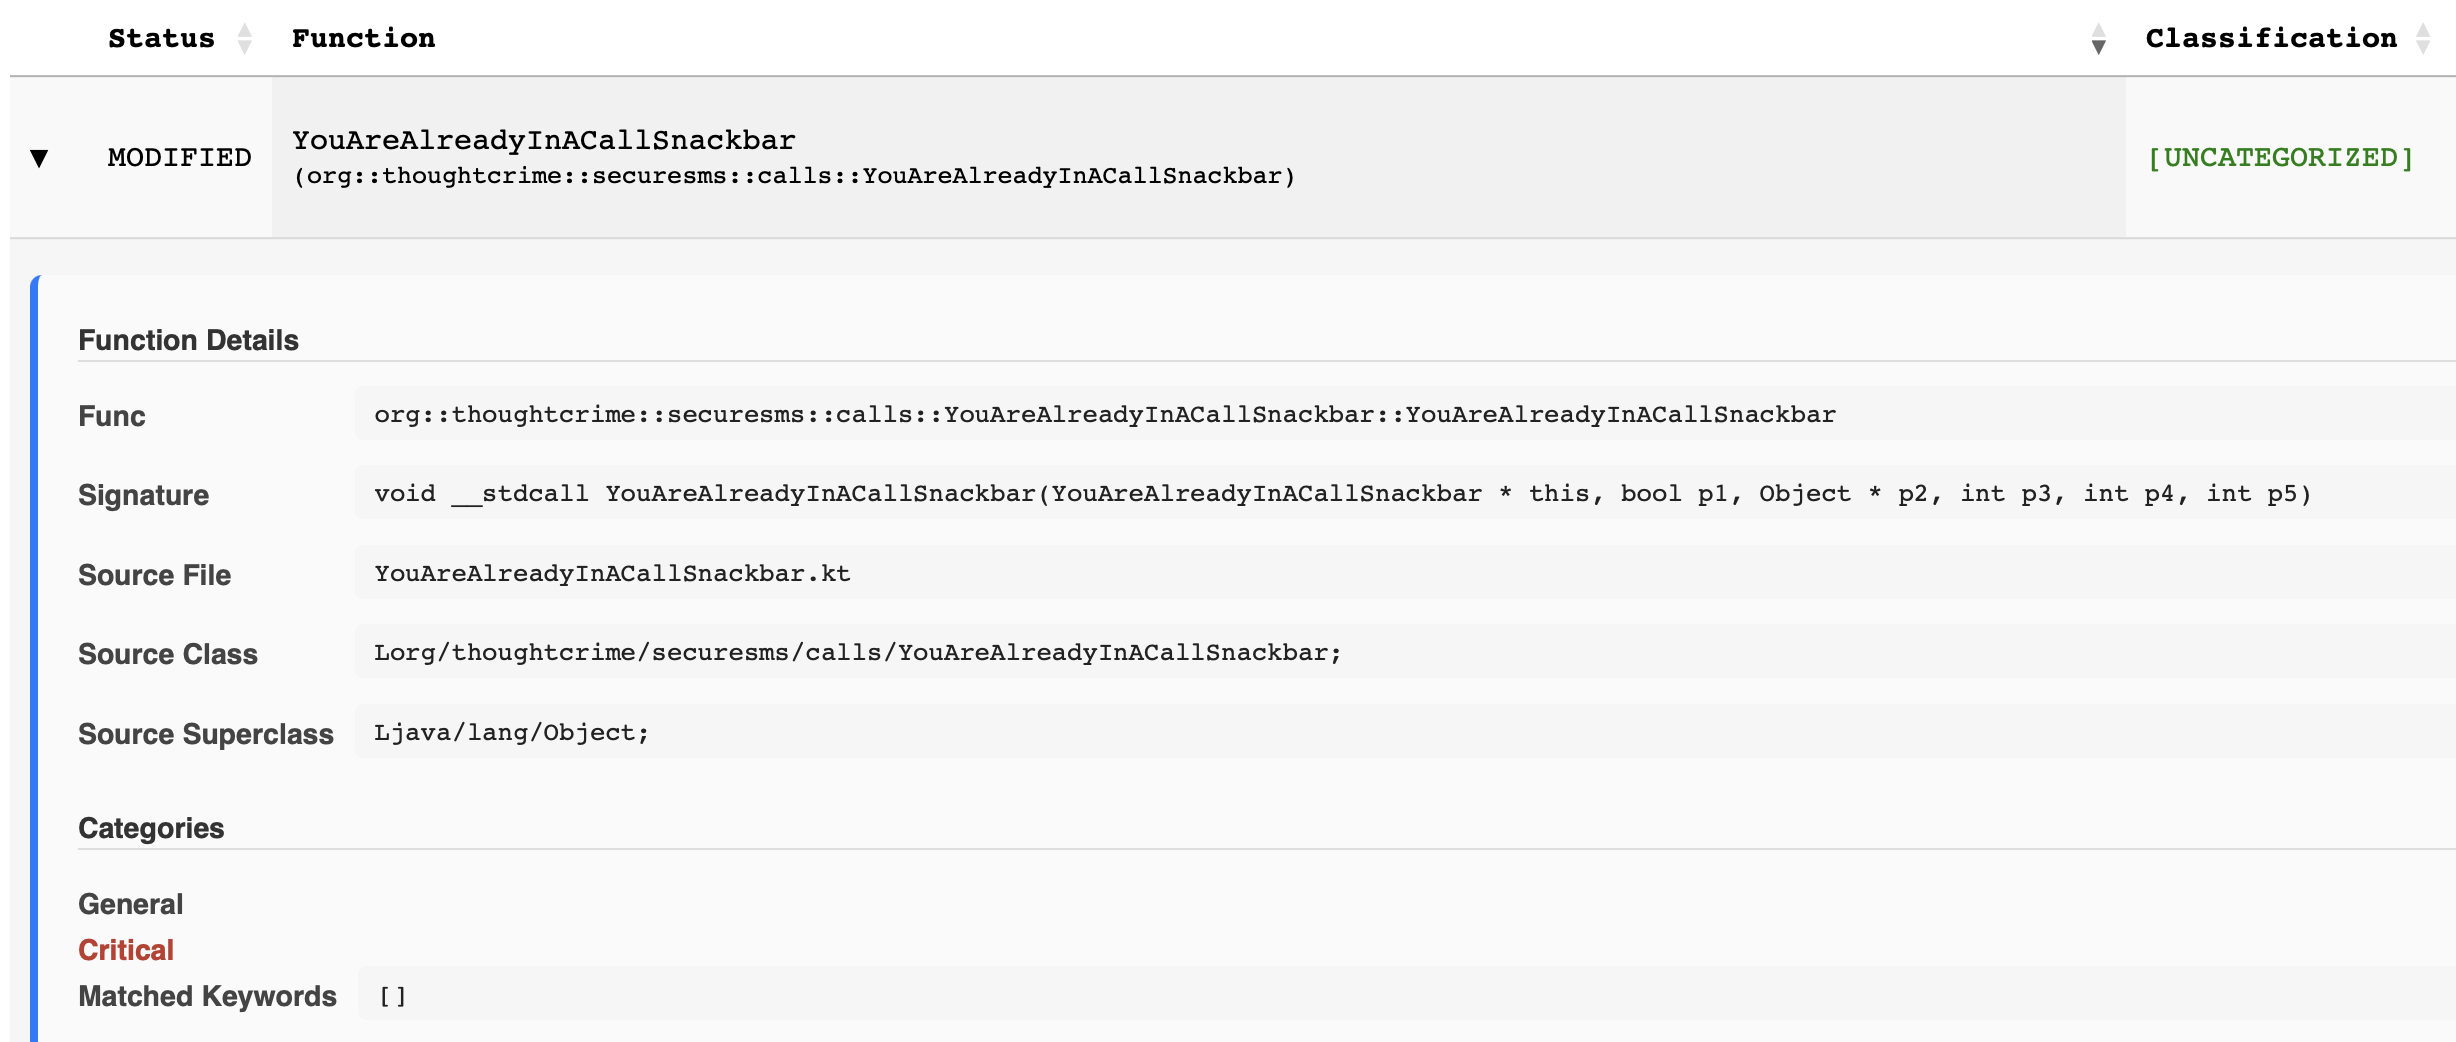
\includegraphics[width=1\linewidth]{figures/results/report_screenshots/method_detailed_1.png}
    \caption{Detailed view of a single change}
    \label{fig:pipeline_detailedview1}
\end{figure}

\begin{figure}[H]
    \centering
    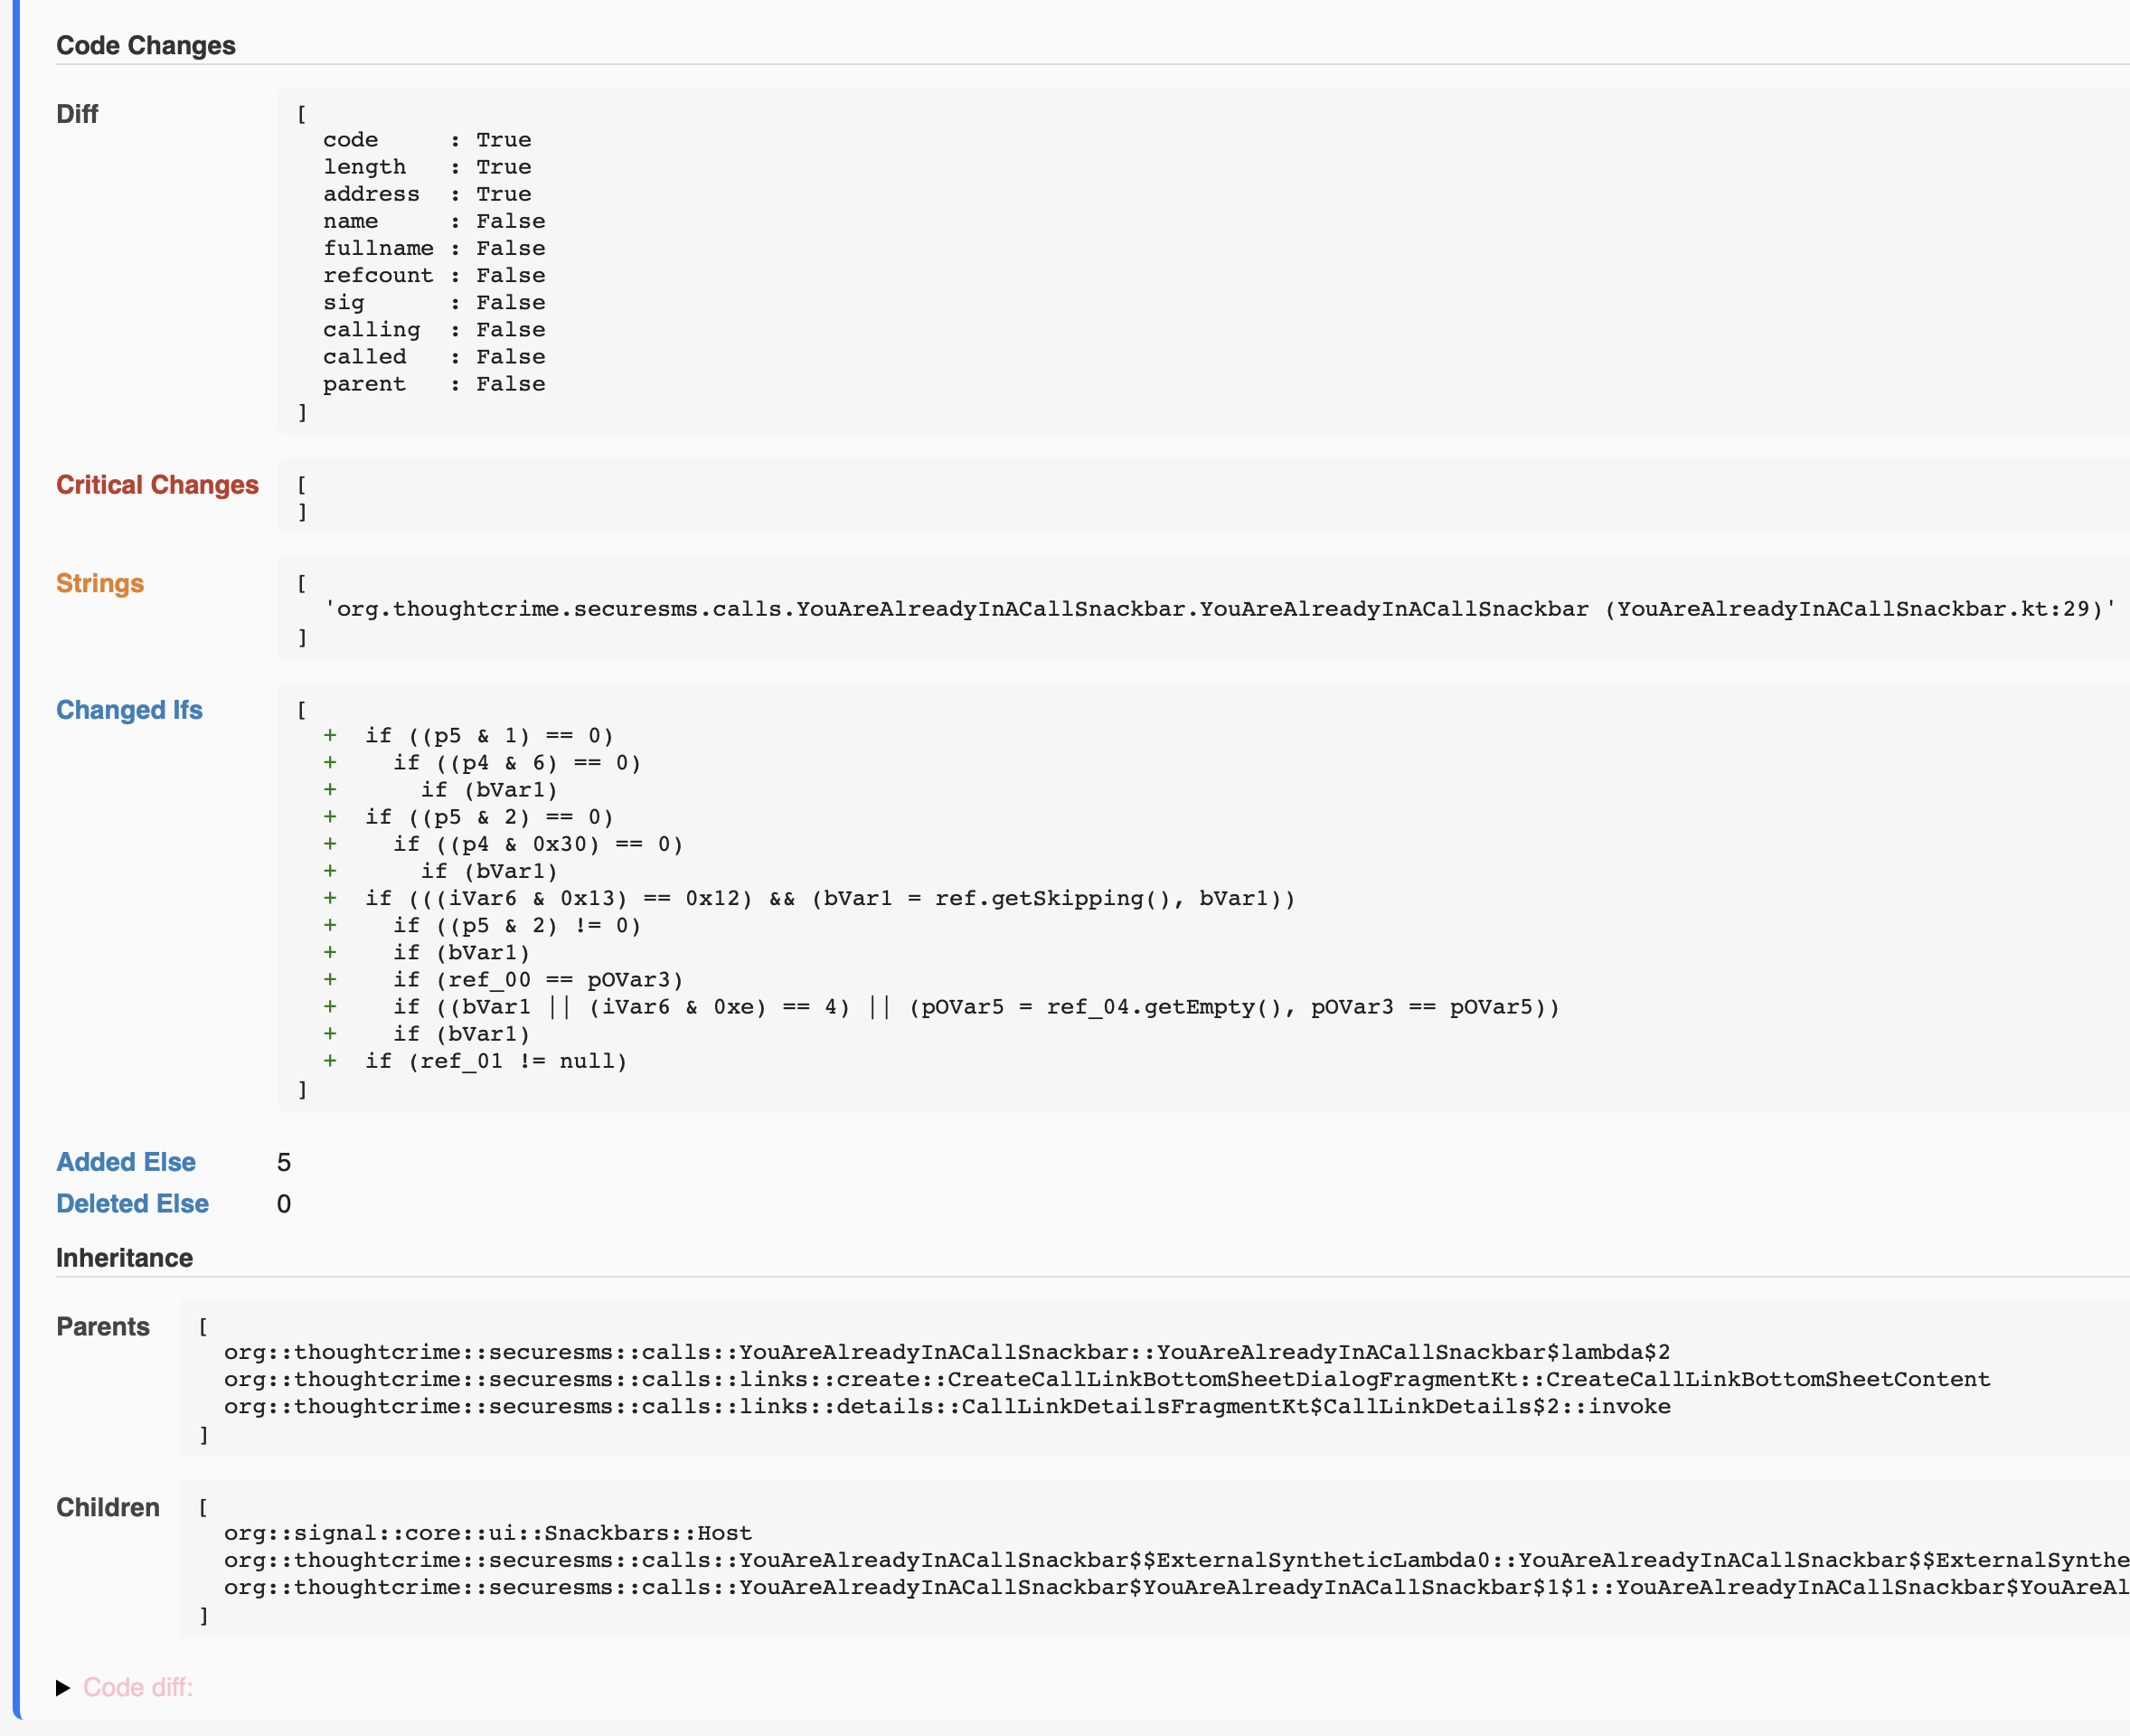
\includegraphics[width=1\linewidth]{figures/results/report_screenshots/method_detailed_2.png}
    \caption{Continued detailed view of a single change}
    \label{fig:pipeline_detailedview2}
\end{figure}

The HTML report offers a feature for comparing decompiled Ghidra code, providing a view of changes between the "old" and "new" versions of the analyzed binaries. This comparison is accessible directly within the detailed view of each detected change. The code differences are highlighted using color coding—the "old" version appears in red, while the "new" version is in green. This visual contrast makes it easy to identify added, removed, or modified lines of code, providing a clear understanding of how the code has changed. Figure \ref{fig:pipeline_codecomparison} demonstrates this code comparison feature.

The report also includes a dark mode option, which can be toggled using a button at the top of the page, and Figure \ref{fig:pipeline_darkmode} presents an example of the report displayed in dark mode.

\begin{figure}[H]
    \centering
    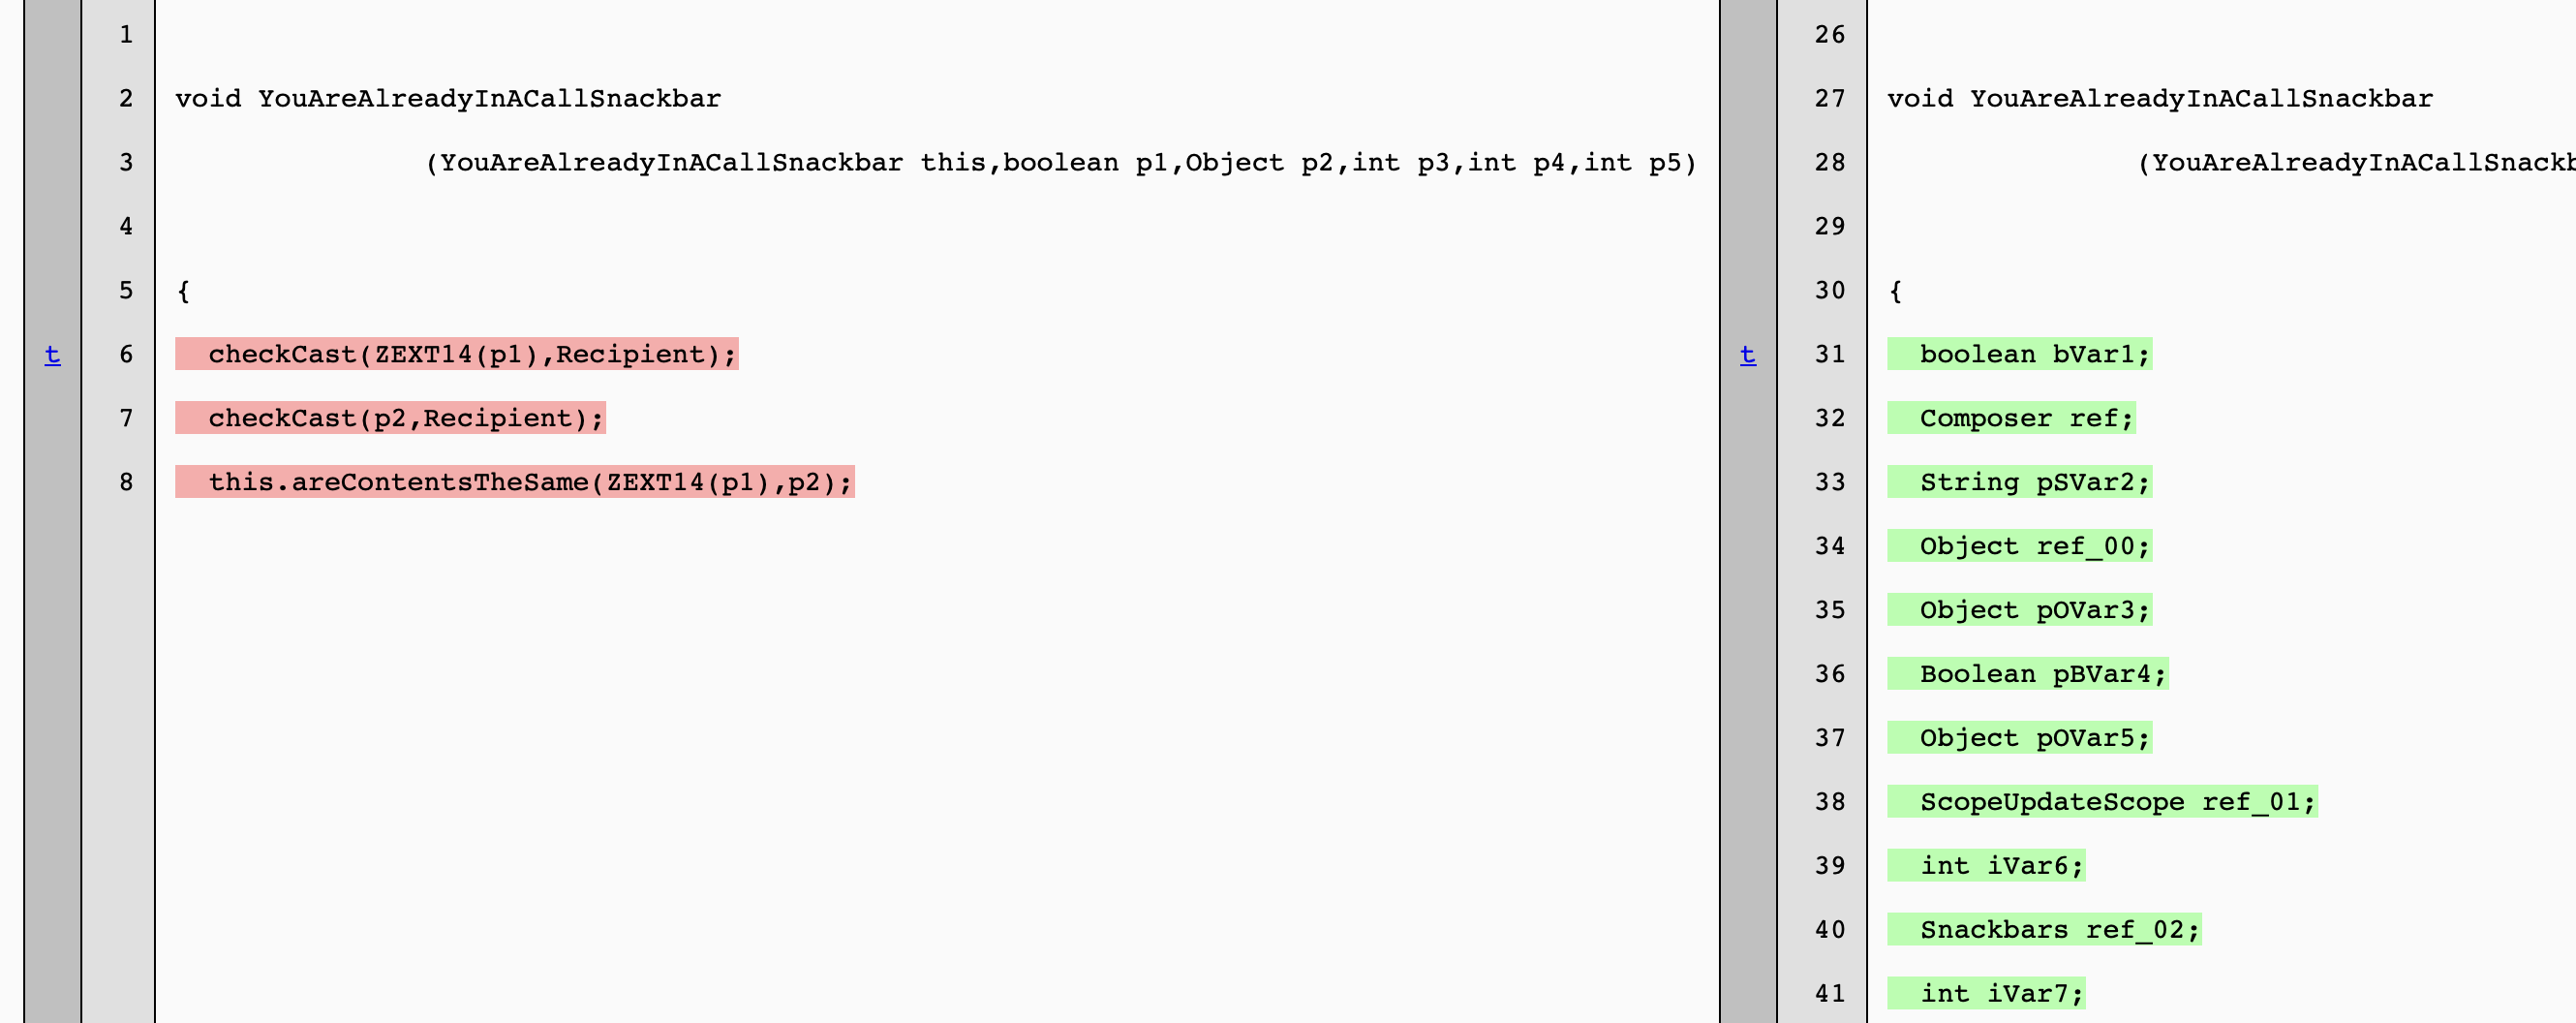
\includegraphics[width=1\linewidth]{figures/results/report_screenshots/method_detailed_code_comparison.png}
    \caption{Decompiled Ghidra code comparison}
    \label{fig:pipeline_codecomparison}
\end{figure}

\begin{figure}[H]
    \centering
    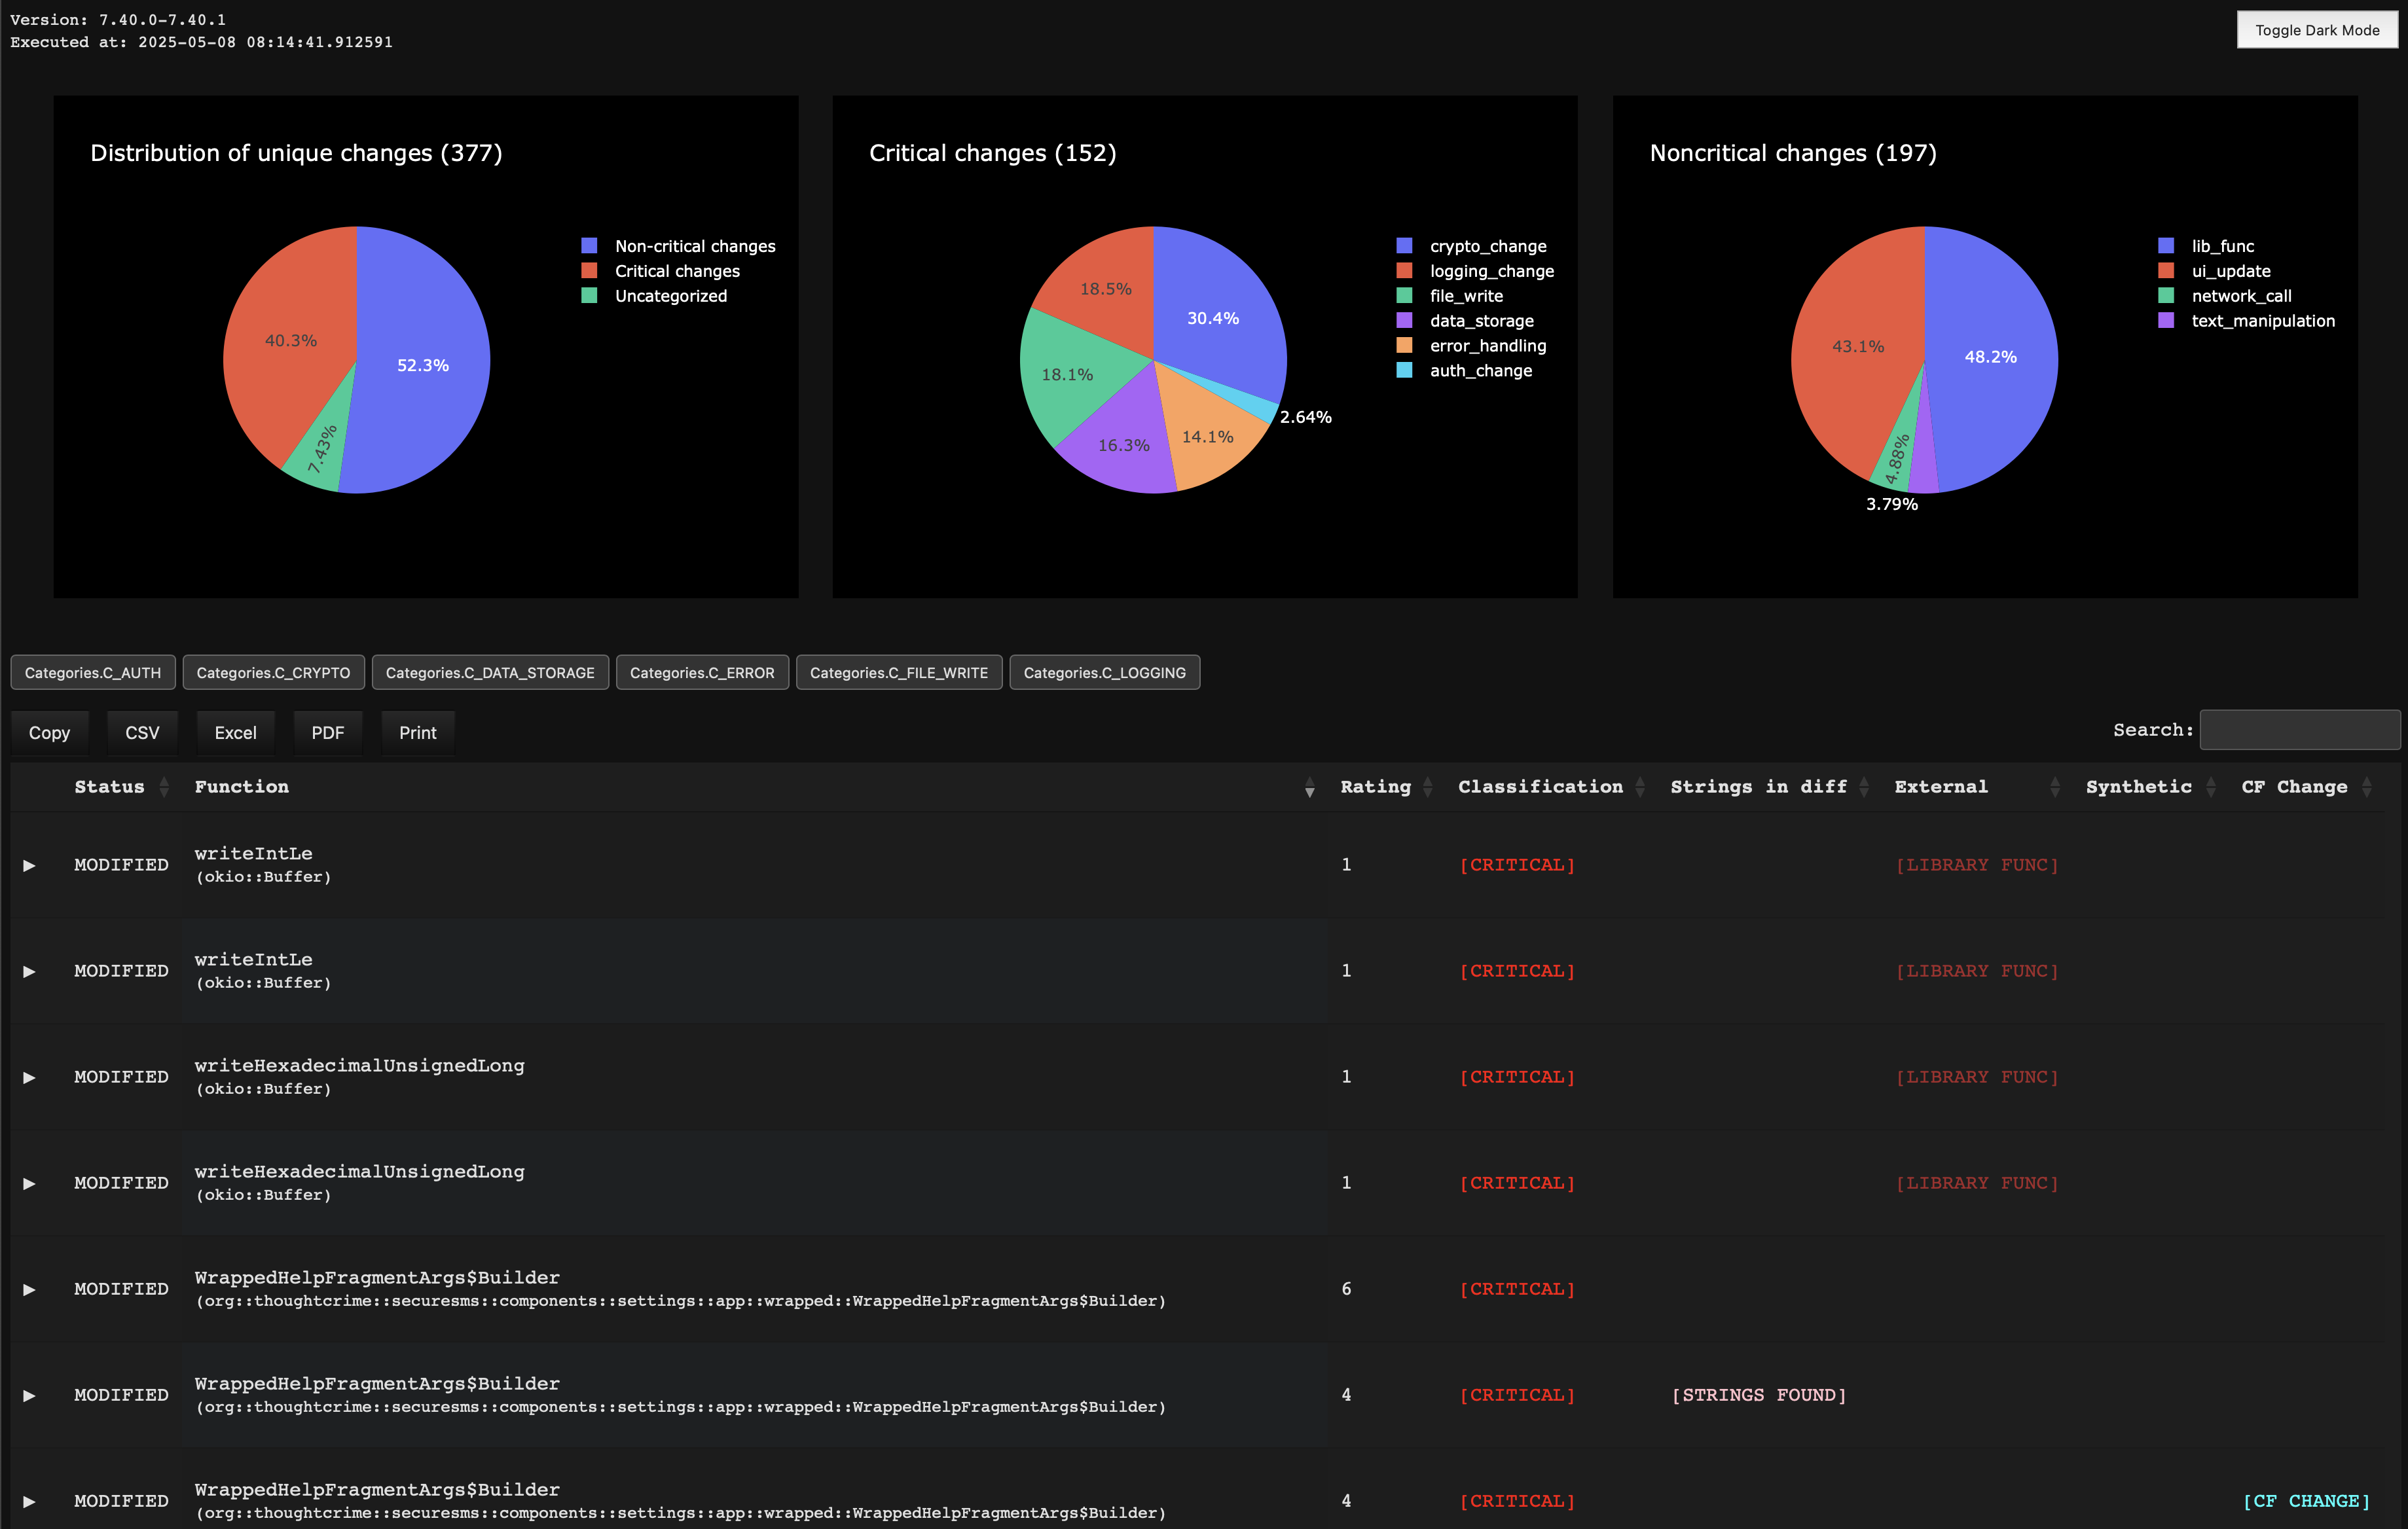
\includegraphics[width=1\linewidth]{figures/results/report_screenshots/feature_darkmode.png}
    \caption{Darkmode enabled}
    \label{fig:pipeline_darkmode}
\end{figure}


\newpage
\section{Categorization Results}
This section presents the results obtained from analyzing three different versions of the Signal Android application using the tool developed in this thesis. The selected versions, summarized in Table \ref{tab:release_overview}, are sourced from Signal's official Android GitHub repository \cite{githubSignal}. Additionally, Table \ref{tab:run_time} provides an overview of the tool’s runtime performance for each version analysis, including key metrics such as analysis duration and the number of detected changes.

\begin{note}
    Partial Analysis of Version Diff B\\
    \noindent
    For version diff B, only a subset of the GitHub changes was manually reviewed during the analysis. Consequently, while Table \ref{tab:run_time} lists a higher number of detected changes for version diff B compared to version diff A, the actual volume of analyzed result data presented in this chapter is smaller for version diff B. This discrepancy is due to the limited scope of the manual review.
\end{note}


\subsection{Understanding the Pipeline Analysis}
The pipeline analysis in this section focuses on three key aspects:

\begin{description}
    \item[Change Detection] Identifying individual changes between the two versions of the Signal application. Each change is defined as a single method-level modification detected between the compared versions.

    \item[Status Classification] Assigning each detected change to one of three status categories: Critical, Non-critical, or Uncategorized. These categories help determine the significance of each change.

    \item[Functional Categorization] Labeling each detected change with one or more functional categories, such as \codebox{Data storage}, \codebox{UI update}, or \codebox{Authentication}. Unlike the status classification, a single change can belong to multiple functional categories.
\end{description}

It is important to note that the total number of detected changes reflects the unique modifications found, while the count of changes in each category may exceed this total because some changes are assigned to multiple categories. This distinction ensures a clear understanding of the results and their classification.

\begin{table}[H]
  \centering
  \begin{tabular}{@{} c c c c c c c @{}}
    \toprule
    \textbf{Version diff} & \textbf{Base} & \textbf{Target} & \textbf{Release date} & \textbf{Commits} & \textbf{File changed} \\ \midrule
    A & v7.30.2 & v7.31.0 & 2025-01-23 & 46 & 171 \\
    B & v7.34.2 & v7.35.0 & 2025-02-21 & 33 & 173 \\
    C & v7.40.0 & v7.40.1 & 2025-04-11 & 12 & 85 \\ \bottomrule
  \end{tabular}
  \caption{Overview of version diffs from Signal's Android GitHub repository \cite{githubSignal}}
  \label{tab:release_overview}
\end{table}


\begin{note}
    Failed .dex File Analysis.\\
    \noindent
    The column labeled "Failed .dex files" in Table \ref{tab:run_time} indicates whether the pipeline (specifically Ghidra) encountered issues analyzing any .dex files. If any .dex files could not be properly analyzed, this can impact the accuracy of the results for that version diff. Missing or failed .dex file analysis reduces the likelihood of detecting all changes and can affect classification performance. This challenge is further discussed in Section \ref{sec:discussion-results}.
\end{note}


\begin{table}[H]
  \centering
  \begin{tabular}{@{} c c c c l @{}}
    \toprule
    \textbf{Version diff} & \textbf{Run time} & \textbf{Apk size} & \textbf{Detected changes} & \textbf{Failed .dex files} \\ \midrule
    A & 20m 45s & 99.3 MB  & 1677 &  \\
    B & 21m 43s & 100 MB & 2386 & classes2.dex \& classes5.dex \\
    C & 21m 25s & 102 MB & 377 & classes2.dex \\ \bottomrule
  \end{tabular}
  \caption{Runtime comparison of the different version diffs. Execution time captured on a MacBook Pro with M1 Pro chip}
  \label{tab:run_time}
\end{table}

\subsection{Manual Evaluation Process}
\label{sec:res:categorization_result:manual_evaluation_process}

To accurately assess the performance of the pipeline’s categorization, a manual evaluation process was conducted. This process involved carefully reviewing the source code for each version difference (diff) and comparing the results with the analysis generated by the pipeline. The manual evaluation followed these structured steps:

\begin{enumerate}
    \item \textbf{Identify Change Types:} For each detected change, it was determined whether it was an addition, modification, or deletion when comparing the new version of the code with the old version.

    \item \textbf{Assign Functional Categories:} Each identified change was categorized based on its nature and functionality. If a change matched any of the predefined functional categories (e.g., Data Storage, UI Update, Authentication), it was labeled accordingly. If none of the categories were applicable, the change was marked as \textit{Uncategorized}.

    \item \textbf{Compare with Pipeline Results:} Each manually identified change was cross-referenced with the HTML report generated by the pipeline. This comparison checked whether the pipeline correctly detected the change, accurately classified it, and assigned the appropriate categories. Any changes detected manually but missing from the pipeline report were also noted.
\end{enumerate}

The results of this manual evaluation are crucial because they serve as a benchmark for assessing the pipeline's accuracy. Although the manual analysis was conducted separately from the pipeline, it reflects the intended behavior of the tool and provides a standard for comparison. 


\subsection{Understanding Correct and Incorrect Classification}
\label{sec:result:understanding_correct_incorrect}
\begin{description}
    \item[Correct Category Classification] This means that the pipeline correctly assigned all categories identified during the manual analysis. Even if the pipeline assigned extra categories, it is still considered correct as long as it includes all the manually identified categories.

    \item[Incorrect Category Classification] This occurs when the pipeline fails to include all categories assigned during the manual analysis. This can happen if the pipeline detects only a subset of the manually assigned categories or if it entirely misses the correct categories.
\end{description}

Further discussion regarding the reliability of these manually gathered results can be found in Section~\ref{sec:discussion-results}.

\subsection{Pipeline Accuracy}

The accuracy of the pipeline’s categorization is determined by comparing its results with the manually reviewed source code analysis \cite{githubSignal}. This comparison helps measure how well the pipeline identifies changes, classifies them, and assigns appropriate categories. The results of this accuracy evaluation are summarized in Tables~\ref{tab:accuracy_A}, \ref{tab:accuracy_B}, and \ref{tab:accuracy_C}.

\noindent
The following metrics are used to evaluate pipeline accuracy:

\begin{description}
    \item[Changes Detected:] The proportion of changes in the source code that were correctly identified by the pipeline. It reflects how effectively the pipeline detects differences between software versions.

    \item[Correct Change Status:] The percentage of changes where the pipeline correctly identified the type of change (addition, modification, or deletion) as compared with the source code.

    \item[Correctly Set Categories:] The proportion of changes where the pipeline correctly assigned the same functional categories as those identified in the manual analysis. If the pipeline assigns all manually identified categories (even with additional categories), the classification is considered correct. However, if it assigns only a subset of the categories identified manually, the classification is marked as incorrect.
\end{description}

It is important to note that these accuracy metrics exclude any changes that the pipeline failed to detect due to limitations in Ghidriff's binary analysis capabilities. This ensures that the evaluation focuses solely on the changes that were actually detected.


\begin{table}[H]
    \centering
    \begin{tabular}{l l}
        \toprule
        \textbf{Metric} & \textbf{Accuracy} \\
        \midrule
        Changes detected & 96.4\% \\
        Correct change status & 84.5\% \\
        Correctly set categories & 85.7\% \\
        \textit{\ \ \ \ \ \ \ \ Critical categories} & 84.2\% \\
        \textit{\ \ \ \ \ \ \ \ Non-critical categories} & 88.9\% \\
        \bottomrule
    \end{tabular}
    \caption{Accuracy metrics for version diff A}
    \label{tab:accuracy_A}
\end{table}

\begin{table}[H]
    \centering
    \begin{tabular}{l l}
        \toprule
        \textbf{Metric} & \textbf{Accuracy} \\
        \midrule
        Changes detected                 & 75\% \\
        Correct change status            & 57.1\% \\
        Correctly set categories & 60.7\% \\
        \textit{\ \ \ \ \ \ \ \ Critical categories} & 56.25\% \\
        \textit{\ \ \ \ \ \ \ \ Non-critical categories} & 66.7\% \\
        \bottomrule
    \end{tabular}
    \caption{Accuracy metrics for version diff B}
    \label{tab:accuracy_B}
\end{table}

\begin{table}[H]
    \centering
    \begin{tabular}{l l}
        \toprule
        \textbf{Metric} & \textbf{Accuracy} \\
        \midrule
        Changes detected                 & 92.9\% \\
        Correct change status            & 82.1\% \\
        Correctly set categories & 53.6\% \\
        \textit{\ \ \ \ \ \ \ \ Critical categories} & 75\% \\
        \textit{\ \ \ \ \ \ \ \ Non-critical categories} & 50\% \\
        \bottomrule
    \end{tabular}
    \caption{Accuracy metrics for version diff C}
    \label{tab:accuracy_C}
\end{table}




%%%% Categorization distribution %%%%
\subsection{Categorization Distributions}

This section provides a detailed analysis of the distribution of categorized changes identified during the pipeline analysis. Specifically, it examines the overall distribution of changes across different categories (Critical, Non-Critical, and Uncategorized) and evaluates the accuracy of these classifications by comparing the ratio of \textit{correct} versus \textit{incorrect} category assignments.

\subsubsection{Distribution of Unique Changes}

The pipeline analysis categorizes each detected change—each method or function listed in the report—into one of three main categories: \textit{Critical}, \textit{Non-Critical}, or \textit{Uncategorized}. Critical changes represent modifications that directly impact the core functionality of the application. Non-critical changes are those that do not significantly affect the application’s main operations, and \textit{uncategorized} changes are those that do not match any of the predefined categories.

The overall distribution of these categories is visually represented using pie charts in Figures~\ref{fig:categorization_A}, \ref{fig:categorization_B}, and \ref{fig:categorization_C}. Each pie chart illustrates the proportion of changes that fall under each category for the three analyzed versions. This graphical representation provides an overview of the prevalence of each category across the analyzed versions, helping to identify patterns and trends.

Since software releases vary in size and scope, deriving results from the distribution of \textit{Critical} and \textit{non-critical} changes across versions is not meaningful. However, aggregating the number of \textit{Uncategorized} changes among all three versions reveals that only 3.3\%  of uniquely detected changes fall outside the defined categories.

\begin{figure}[H]
    \centering
    \resizebox{0.92\textwidth}{!}{%
        \begin{tikzpicture}
        \path[%
            % style options
            dc sector/.append style={shift={(\MedA:5pt)}}, % shift all sectors
            dc dtag/.append style={},
            dc legend/.append style={text width=3cm, align=right},
            every pin/.style={fill=\Cj,draw=\Cj!50!black,thick},
            % diagram options
            /DiagCirc/.cd,
            value list={1311/Critical,343/Non-critical,23/Uncategorized},
            color list={"color10","color11","color12"},
            angle max=180,             % semi-circular
            angle corr={0,0,0,0,0},    % correct round angle error
            legend=\N\ :\hfill \V,     % custom legend
            factor=.9,
            percent corr={0,0,0,0,0}, % correct round percent error
            shift sector={0,0,0,0,0}, % shift individual sector
            tags=\P,                   % custom sector nodes
            sup loop={% custom features :       
                %--- pin directions just for THIS figure --------------
                %   slice 0   slice 1        slice 2
                \def\Pin{{87,  100,           150}}
                %   ↑   moved Critical up to 80° so it clears the legend
                \pgfmathparse{array(\Pin,\j)}
                \edef\Pinj{\pgfmathresult}
                \node[pin=\Pinj:\N] at (DC\j) {};
                },
            diagram] ;
        \end{tikzpicture}
    }
    \caption{Distribution of categorizations from version diff A}
    \label{fig:categorization_A}
\end{figure}

\begin{figure}[H]
    \centering
    \resizebox{0.92\textwidth}{!}{%
        \begin{tikzpicture}
        \path[%
            % style options
            dc sector/.append style={shift={(\MedA:5pt)}}, % shift all sectors
            dc dtag/.append style={},
            dc legend/.append style={text width=3cm, align=right},
            every pin/.style={fill=\Cj,draw=\Cj!50!black,thick},
            % diagram options
            /DiagCirc/.cd,
            value list={1341/Critical,948/Non-critical,97/Uncategorized},
            color list={"color10","color11","color12"},
            angle max=180,             % semi-circular
            angle corr={0,0,0,0,0},    % correct round angle error
            legend=\N\ :\hfill \V,     % custom legend
            factor=.9,
            percent corr={0,0,0,0,0}, % correct round percent error
            shift sector={0,0,0,0,0}, % shift individual sector
            tags=\P,                   % custom sector nodes
            sup loop={% custom features :       
                %--- pin directions just for THIS figure --------------
                %   slice 0   slice 1        slice 2
                \def\Pin{{87,  100,           150}}
                %   ↑   moved Critical up to 80° so it clears the legend
                \pgfmathparse{array(\Pin,\j)}
                \edef\Pinj{\pgfmathresult}
                \node[pin=\Pinj:\N] at (DC\j) {};
                },
            diagram] ;
        
        \end{tikzpicture}
    }
    \caption{Distribution of categorizations from version diff B}
    \label{fig:categorization_B}
\end{figure}

\begin{figure}[H]
    \centering
    \resizebox{0.92\textwidth}{!}{%
        \begin{tikzpicture}
        \path[%
            % style options
            dc sector/.append style={shift={(\MedA:5pt)}}, % shift all sectors
            dc dtag/.append style={},
            dc legend/.append style={text width=3cm, align=right},
            every pin/.style={fill=\Cj,draw=\Cj!50!black,thick},
            % diagram options
            /DiagCirc/.cd,
            value list={152/Critical,197/Non-critical,28/Uncategorized},
            color list={"color10","color11","color12"},
            angle max=180,             % semi-circular
            angle corr={0,0,0,0,0},    % correct round angle error
            legend=\N\ :\hfill \V,     % custom legend
            factor=.9,
            percent corr={0,0,0,0,0}, % correct round percent error
            shift sector={0,0,0,0,0}, % shift individual sector
            tags={%
                \P                   % custom sector nodes
            },
            sup loop={% custom features :       
                %--- pin directions just for THIS figure --------------
                %   slice 0   slice 1        slice 2
                \def\Pin{{330,  100,           150}}
                %   ↑   moved Critical up to 80° so it clears the legend
                \pgfmathparse{array(\Pin,\j)}
                \edef\Pinj{\pgfmathresult}
                \node[pin=\Pinj:\N] at (DC\j) {};
            },
            diagram] ;
        
        \end{tikzpicture}
    }
    \caption{Distribution of categorizations from version diff C}
    \label{fig:categorization_C}
\end{figure}



% critical cat piecharts %
\subsubsection{Critical Categorization Distribution}
The critical changes identified during the pipeline analysis are divided into six predefined categories, previously introduced in Section~\ref{sec:method:changes_to_categorize}. These categories represent specific types of changes that are considered highly impactful, directly affecting the application's functionality, security, or data management. 
A detailed breakdown of the distribution of detected hits for each critical category is presented in Figures~\ref{fig:critical_changes_A}, \ref{fig:critical_changes_B}, and \ref{fig:critical_changes_C}. These figures show the number of times each critical category was assigned to a detected change across the three analyzed version differences (A, B, and C).
It is important to note that the term "hit" does not directly correspond to a unique change. A single detected change can belong to multiple categories, meaning it can generate multiple hits if categorized under several critical categories. This allows for a more comprehensive view of how changes are categorized, capturing the full scope of their impact.


\begin{figure}[H]
    \centering
    \resizebox{0.8\textwidth}{!}{%
        \begin{tikzpicture}
        \path[%
            % style options
            dc sector/.append style={shift={(\MedA:5pt)}}, % shift all sectors
            dc dtag/.append style={},
            dc legend/.append style={text width=3.5cm, align=right},
            every pin/.style={fill=\Cj,draw=\Cj!50!black,thick},
            % diagram options
            /DiagCirc/.cd,
            value list={
                837/Data storage,
                340/Authentication,
                609/Logging,
                462/Error handling,
                345/File write,
                175/Cryptographic
            },
            angle max=360,             % semi-circular
            angle corr={0,0,0,0,0,0},    % correct round angle error
            legend=\N\ :\hfill \V,     % custom legend
            factor=.9,
            percent corr={0,0,0,0,0,0}, % correct round percent error
            shift sector={0,0,0,0,0,0}, % shift individual sector
            tags={%
                \P                   % custom sector nodes
            },
            sup loop={% custom features :       
                %--- pin directions just for THIS figure --------------
                %   slice 0, slice 1, ..., 
                \def\Pin{{85, 110, 120, 180, 320, 340}}
                %   ↑   moved Critical up to 80° so it clears the legend
                \pgfmathparse{array(\Pin,\j)}
                \edef\Pinj{\pgfmathresult}
                \node[pin=\Pinj:\N] at (DC\j) {};
            },
            diagram] ;
        
        \end{tikzpicture}
    }
    \caption{Distribution of hits for each critical category from analysis of version diff A}
    \label{fig:critical_changes_A}
\end{figure}

\begin{figure}[H]
    \centering
    \resizebox{0.8\textwidth}{!}{%
        \begin{tikzpicture}
        \path[%
            % style options
            dc sector/.append style={shift={(\MedA:5pt)}}, % shift all sectors
            dc dtag/.append style={},
            dc legend/.append style={text width=3.5cm, align=right},
            every pin/.style={fill=\Cj,draw=\Cj!50!black,thick},
            % diagram options
            /DiagCirc/.cd,
            value list={
                455/Data storage,
                355/Authentication,
                732/Logging,
                586/Error handling,
                452/File write,
                127/Cryptographic
            },
            angle max=360,             % semi-circular
            angle corr={0,0,0,0,0,0},    % correct round angle error
            legend=\N\ :\hfill \V,     % custom legend
            factor=.9,
            percent corr={0,0,0,0,0,0}, % correct round percent error
            shift sector={0,0,0,0,0,0}, % shift individual sector
            tags={%
                \P                   % custom sector nodes
            },
            sup loop={% custom features :       
                %--- pin directions just for THIS figure --------------
                %   slice 0, slice 1, ..., 
                \def\Pin{{240, 0, 120, 200, 320, 340}}
                %   ↑   moved Critical up to 80° so it clears the legend
                \pgfmathparse{array(\Pin,\j)}
                \edef\Pinj{\pgfmathresult}
                \node[pin=\Pinj:\N] at (DC\j) {};
            },
            diagram] ;
        
        \end{tikzpicture}
    }
    \caption{Distribution of hits for each critical category from analysis of version diff B}
    \label{fig:critical_changes_B}
\end{figure}

\begin{figure}[H]
    \centering
    \resizebox{0.8\textwidth}{!}{%
        \begin{tikzpicture}
        \path[%
            % style options
            dc sector/.append style={shift={(\MedA:5pt)}}, % shift all sectors
            dc dtag/.append style={},
            dc legend/.append style={text width=3cm, align=right},
            every pin/.style={fill=\Cj,draw=\Cj!50!black,thick},
            % diagram options
            /DiagCirc/.cd,
            value list={
                37/Data storage,
                6/Authentication,
                42/Logging,
                32/Error handling,
                41/File write,
                69/Cryptographic
            },
            angle max=360,             % semi-circular
            angle corr={0,0,0,0,0,0},    % correct round angle error
            legend=\N\ :\hfill \V,     % custom legend
            factor=.9,
            percent corr={0,0,0,0,0,0}, % correct round percent error
            shift sector={0,0,0,0,0,0}, % shift individual sector
            tags={%
                \P                   % custom sector nodes
            },
            sup loop={% custom features :       
                %--- pin directions just for THIS figure --------------
                %   slice 0, slice 1, ..., 
                \def\Pin{{240, 70, 170, 160, 230, 330}}
                %   ↑   moved Critical up to 80° so it clears the legend
                \pgfmathparse{array(\Pin,\j)}
                \edef\Pinj{\pgfmathresult}
                \node[pin=\Pinj:\N] at (DC\j) {};
            },
            diagram] ;
        
        \end{tikzpicture}
    }
    \caption{Distribution of hits for each critical category from analysis of version diff C}
    \label{fig:critical_changes_C}
\end{figure}

An analysis of Figures~\ref{fig:critical_changes_A}, \ref{fig:critical_changes_B}, and \ref{fig:critical_changes_C} reveals that the distribution of critical categories remains relatively consistent across the three version differences, despite substantial variations in the total number of detected changes for each version. This consistency suggests that the types of critical changes detected are generally similar, even though the code modifications and their underlying purposes may differ significantly between versions.

This observation can be interpreted in two contrasting ways. On the one hand, it may be viewed as a potential limitation of the categorization process, as it could imply that the pipeline detects similar categories regardless of the actual nature of the changes. Given that different versions of an application are unlikely to have identical change patterns, this uniform distribution might be seen as a sign of overgeneralization.
On the other hand, this consistency can also be considered a strength of the analysis. It demonstrates that even minor modifications in the source code can lead to distinct execution paths, each captured and categorized by the pipeline. This ability to detect and classify a wide range of changes—regardless of their scale—highlights the sensitivity and thoroughness of the tool.
A more detailed discussion of this observation, including its implications and potential improvements, is provided in Section~\ref{sec:discussion-results}.








% noncritical cat dist %
\subsubsection{Non-critical categorization distribution}
The non-critical changes identified during the pipeline analysis are categorized into four distinct categories, as previously introduced in Section~\ref{sec:method:changes_to_categorize}. These categories capture modifications that, while relevant, do not directly impact the core functionality, security, or data handling of the application. Such changes typically include user interface updates, logging adjustments, and other non-essential modifications.
A detailed breakdown of the distribution of hits within each non-critical category is presented in Figures~\ref{fig:noncritical_changes_A}, \ref{fig:noncritical_changes_B}, and \ref{fig:noncritical_changes_C}. These figures illustrate how frequently each non-critical category was assigned across the three versions (A, B, and C), providing a clear view of how such changes are distributed in each analyzed version.
It is important to clarify that the term "hit" in this context does not directly correspond to a unique change. A single detected change may be assigned to multiple categories, resulting in multiple hits. For instance, a change that affects both user interface elements and logging functionality would be counted as a hit in both categories. This approach allows for a more comprehensive understanding of the nature of the detected changes.


\begin{figure}[H]
    \centering
    \resizebox{0.92\textwidth}{!}{%
        \begin{tikzpicture}
        \path[%
            % style options
            dc sector/.append style={shift={(\MedA:5pt)}}, % shift all sectors
            dc dtag/.append style={},
            dc legend/.append style={text width=3.5cm, align=right},
            every pin/.style={fill=\Cj,draw=\Cj!50!black,thick},
            % diagram options
            /DiagCirc/.cd,
            value list={
                124/Network call,
                816/UI update,
                193/Library function,
                27/Text manipulation
            },
            color list={"color6","color7","color8","color9"},
            angle max=180,             % semi-circular
            angle corr={0,0,0,0,0,0},    % correct round angle error
            legend=\N\ :\hfill \V,     % custom legend
            factor=.9,
            percent corr={0,0,0,0,0,0}, % correct round percent error
            shift sector={0,0,0,0,0,0}, % shift individual sector
            tags={%
                \P                   % custom sector nodes
            },
            sup loop={% custom features :       
                %--- pin directions just for THIS figure --------------
                %   slice 0, slice 1, ..., 
                \def\Pin{{350, 170, 130, 160}}
                %   ↑   moved Critical up to 80° so it clears the legend
                \pgfmathparse{array(\Pin,\j)}
                \edef\Pinj{\pgfmathresult}
                \node[pin=\Pinj:\N] at (DC\j) {};
            },
            diagram] ;
        
        \end{tikzpicture}
    }
    \caption{Distribution of hits for each non-critical category from analysis of version diff A}
    \label{fig:noncritical_changes_A}
\end{figure}

\begin{figure}[H]
    \centering
    \resizebox{0.92\textwidth}{!}{%
        \begin{tikzpicture}
        \path[%
            % style options
            dc sector/.append style={shift={(\MedA:5pt)}}, % shift all sectors
            dc dtag/.append style={},
            dc legend/.append style={text width=3.5cm, align=right},
            every pin/.style={fill=\Cj,draw=\Cj!50!black,thick},
            % diagram options
            /DiagCirc/.cd,
            value list={
                1183/Network call,
                889/UI update,
                1062/Library function,
                197/Text manipulation
            },
            color list={"color6","color7","color8","color9"},
            angle max=180,             % semi-circular
            angle corr={0,0,0,0,0,0},    % correct round angle error
            legend=\N\ :\hfill \V,     % custom legend
            factor=.9,
            percent corr={0,0,0,0,0,0}, % correct round percent error
            shift sector={0,0,0,0,0,0}, % shift individual sector
            tags={%
                \P                   % custom sector nodes
            },
            sup loop={% custom features :       
                %--- pin directions just for THIS figure --------------
                %   slice 0, slice 1, ..., 
                \def\Pin{{330, 170, 120, 160}}
                %   ↑   moved Critical up to 80° so it clears the legend
                \pgfmathparse{array(\Pin,\j)}
                \edef\Pinj{\pgfmathresult}
                \node[pin=\Pinj:\N] at (DC\j) {};
            },
            diagram] ;
        
        \end{tikzpicture}
    }
    \caption{Distribution of hits for each non-critical category from analysis of version diff B}
    \label{fig:noncritical_changes_B}
\end{figure}

\begin{figure}[H]
    \centering
    \resizebox{0.92\textwidth}{!}{%
        \begin{tikzpicture}
        \path[%
            % style options
            dc sector/.append style={shift={(\MedA:5pt)}}, % shift all sectors
            dc dtag/.append style={},
            dc legend/.append style={text width=3.5cm, align=right},
            every pin/.style={fill=\Cj,draw=\Cj!50!black,thick},
            % diagram options
            /DiagCirc/.cd,
            value list={
                18/Network call,
                159/UI update,
                178/Library function,
                14/Text manipulation
            },
            color list={"color6","color7","color8","color9"},
            angle max=180,             % semi-circular
            angle corr={0,0,0,0,0,0},    % correct round angle error
            legend=\N\ :\hfill \V,     % custom legend
            factor=.9,
            percent corr={0,0,0,0,0,0}, % correct round percent error
            shift sector={0,0,0,0,0,0}, % shift individual sector
            tags={%
                \P                   % custom sector nodes
            },
            sup loop={% custom features :       
                %--- pin directions just for THIS figure --------------
                %   slice 0, slice 1, ..., 
                \def\Pin{{10, 88, 120, 160}}
                %   ↑   moved Critical up to 80° so it clears the legend
                \pgfmathparse{array(\Pin,\j)}
                \edef\Pinj{\pgfmathresult}
                \node[pin=\Pinj:\N] at (DC\j) {};
            },
            diagram] ;
        
        \end{tikzpicture}
    }
    \caption{Distribution of hits for each non-critical category from analysis of version diff C}
    \label{fig:noncritical_changes_C}
\end{figure}

The data presented in Figures~\ref{fig:noncritical_changes_A}, \ref{fig:noncritical_changes_B}, and \ref{fig:noncritical_changes_C} reveal a clear pattern: the categories \codebox{UI update} and \codebox{Library function} are the most frequently detected among non-critical changes. This outcome is consistent with the nature of the Signal Android application, which serves as the test subject for this analysis. Given that Signal is a messaging app with a user interface that undergoes frequent updates, it is unsurprising that UI-related changes are detected most often. 

Similarly, the high frequency of the \codebox{Library function} category can be attributed to Signal’s reliance on numerous external libraries. Any upstream updates or modifications within these libraries are automatically registered as changes during the analysis. This means that even if the Signal application code itself remains unchanged, updates in the external libraries it depends on are still captured by the pipeline.

\subsubsection{Categories Resulting in \textit{Correct} vs \textit{Incorrect} Categorization}
\label{sec:result:categorization_distributions:categories_resulting_in_correct_incorrect_categorizations}

This section examines the accuracy of the pipeline’s categorization by comparing the number of hits per category that were classified \textit{correctly} versus those that were \textit{incorrectly} categorized. The results are visualized in bar charts in Figures~\ref{fig:category_comparison_A}, \ref{fig:category_comparison_B}, and \ref{fig:category_comparison_C}. 

Each bar chart displays the number of hits (instances) in each category, separated into two groups: correctly categorized and incorrectly categorized. A correct categorization means that the categories assigned by the pipeline match those determined through the manual analysis. An incorrect categorization occurs when the pipeline assigns categories that do not match the manually identified ones. This comparison provides insights into the pipeline’s classification performance for each category.

%, where the Y-axis is the number of assignments, and the X-axis is the category.

\begin{figure}[H]
    \centering
    \begin{tikzpicture}
      \begin{axis}[
        width=15cm,
        height=5.0cm,
        ybar,
        bar width=10pt,
        symbolic x coords={\codebox{UI update},\codebox{Authentication},\codebox{Data storage},\codebox{Logging},\codebox{Network call},\codebox{File write},\codebox{Error handling},\codebox{Cryptographic}},
        xtick=data,
        tick label style={font=\normalsize,rotate=45,anchor=east},
        enlarge x limits=0.05,
        xlabel={Category},
        ylabel={Assignments},
        ymin=0, ymax=50,
        nodes near coords,
        every node near coord/.append style={font=\scriptsize,yshift=2pt},
        axis x line*=bottom,
        axis y line*=left,
        legend style={at={(0.5,0.9)},anchor=south,legend columns=-1},
        legend cell align={left}
      ]
        % ─── Correct (green) ──────────────────────────────
        \addplot[ybar,fill=correct_color] coordinates {
          (\codebox{UI update},45) (\codebox{Authentication},30) (\codebox{Data storage},10) (\codebox{Logging},10) (\codebox{Network call},8)
          (\codebox{File write},0) (\codebox{Error handling},0) (\codebox{Cryptographic},0)
        };
        % ─── Incorrect (red) ─────────────────────────────
        \addplot[ybar,fill=incorrect_color] coordinates {
          (\codebox{UI update},3) (\codebox{Authentication},3) (\codebox{Data storage},3) (\codebox{Logging},5) (\codebox{Network call},1)
          (\codebox{File write},4) (\codebox{Error handling},3) (\codebox{Cryptographic},2)
        };
        \legend{Correct,Incorrect}
      \end{axis}
    \end{tikzpicture}
    \caption{Amount of correctly vs incorrectly assigned categories, per category, for version diff A}
    \label{fig:category_comparison_A}
\end{figure}

\begin{figure}[H]
    \centering
    \begin{tikzpicture}
      \begin{axis}[
        width=15cm,
        height=5.0cm,
        ybar,
        bar width=10pt,
        symbolic x coords={\codebox{UI update},\codebox{Data storage},\codebox{Logging},\codebox{Authentication},\codebox{Error handling},\codebox{Network call},\codebox{File write},\codebox{Cryptographic},\codebox{Text manipulation}},
        xtick=data,
        tick label style={font=\normalsize,rotate=45,anchor=east},
        enlarge x limits=0.05,
        xlabel={Category},
        ylabel={Assignments},
        ymin=0, ymax=10,
        nodes near coords,
        every node near coord/.append style={font=\scriptsize,yshift=2pt},
        axis x line*=bottom,
        axis y line*=left,
        legend style={at={(0.5,0.9)},anchor=south,legend columns=-1},
        legend cell align={left}
      ]
        % ─── Correct (green) ──────────────────────────────
        \addplot[ybar,fill=correct_color] coordinates {
          (\codebox{UI update},7) (\codebox{Data storage},6) (\codebox{Logging},4) (\codebox{Authentication},2) (\codebox{Error handling},2) (\codebox{Network call},2)
          (\codebox{File write},0) (\codebox{Cryptographic},0) (\codebox{Text manipulation},0)
        };
        % ─── Incorrect (red) ─────────────────────────────
        \addplot[ybar,fill=incorrect_color] coordinates {
          (\codebox{UI update},1) (\codebox{Data storage},1) (\codebox{Logging},1) (\codebox{Authentication},0) (\codebox{Error handling},2) (\codebox{Network call},0)
          (\codebox{File write},2) (\codebox{Cryptographic},1) (\codebox{Text manipulation},1)
        };
        \legend{Correct,Incorrect}
      \end{axis}
    \end{tikzpicture}
    \caption{Amount of correctly vs incorrectly assigned categories, per category, for version diff B}
    \label{fig:category_comparison_B}
\end{figure}

\begin{figure}[H]
    \centering
    \begin{tikzpicture}
      \begin{axis}[
        width=15cm,
        height=5.0cm,
        ybar,
        bar width=10pt,
        symbolic x coords={\codebox{UI update},\codebox{Data storage},\codebox{Logging},\codebox{Cryptographic},\codebox{Error handling},\codebox{Network call},\codebox{Uncategorized}},
        xtick=data,
        tick label style={font=\normalsize,rotate=45,anchor=east},
        enlarge x limits=0.05,
        xlabel={Category},
        ylabel={Assignments},
        ymin=0, ymax=15,
        nodes near coords,
        every node near coord/.append style={font=\scriptsize,yshift=2pt},
        axis x line*=bottom,
        axis y line*=left,
        legend style={at={(0.5,0.9)},anchor=south,legend columns=-1},
        legend cell align={left}
      ]
        % ─── Correct (green) ──────────────────────────────
        \addplot[ybar,fill=correct_color] coordinates {
          (\codebox{UI update},13) (\codebox{Data storage},3) (\codebox{Logging},0) (\codebox{Cryptographic},0)
          (\codebox{Error handling},0) (\codebox{Network call},0) (\codebox{Uncategorized},0)
        };
        % ─── Incorrect (red) ─────────────────────────────
        \addplot[ybar,fill=incorrect_color] coordinates {
          (\codebox{UI update},1) (\codebox{Data storage},4) (\codebox{Logging},6) (\codebox{Cryptographic},2)
          (\codebox{Error handling},2) (\codebox{Network call},1) (\codebox{Uncategorized},1)
        };
        \legend{Correct,Incorrect}
      \end{axis}
    \end{tikzpicture}
    \caption{Amount of correctly vs incorrectly assigned categories, per category, for version diff C}
    \label{fig:category_comparison_C}
\end{figure}

From Figures~\ref{fig:category_comparison_A}, \ref{fig:category_comparison_B}, and \ref{fig:category_comparison_C}, it is evident that the category \codebox{UI update} is the most frequently assigned category across all version differences, with a total of 65 assignments. This category shows a substantial lead over the next two most frequently assigned categories: \codebox{Authentication}, which has 32 assignments, and \codebox{Data storage}, which has 19 assignments. 

These three categories—\codebox{UI update}, \codebox{Authentication}, and \codebox{Data storage}—also exhibit the highest correct-to-incorrect ratio, indicating that they are not only frequently assigned but also accurately classified by the pipeline. A more detailed discussion of this performance, including the correct-to-incorrect ratio for each category, is provided later in this chapter in Section~\ref{sec:res:comprehensive_summary}.

\subsection{Keyword Distributions}

This section presents an analysis of the distribution of keywords detected during the pipeline analysis, focusing on their effectiveness in triggering critical or non-critical categories. The results include the total number of hits for each keyword, indicating how often each keyword led to a categorization decision. These hits are further divided into two groups: \textit{correct} and \textit{incorrect}, providing insights into the accuracy of keyword-based classification.

\subsubsection{Keywords Resulting in Critical and Non-Critical Categorizations}

The total number of hits for each keyword that triggered a critical or non-critical classification during the regular-expression analysis is displayed in Figures \ref{fig:commonly_used_words_A}, \ref{fig:commonly_used_words_B}, and \ref{fig:commonly_used_words_C}. Each figure visualizes how frequently each keyword was detected, along with a breakdown of how many of these detections led to correct or incorrect categorizations. This analysis helps identify which keywords are most effective at correctly classifying changes and which may require further refinement to improve accuracy.


\begin{figure}[H]
    \centering
    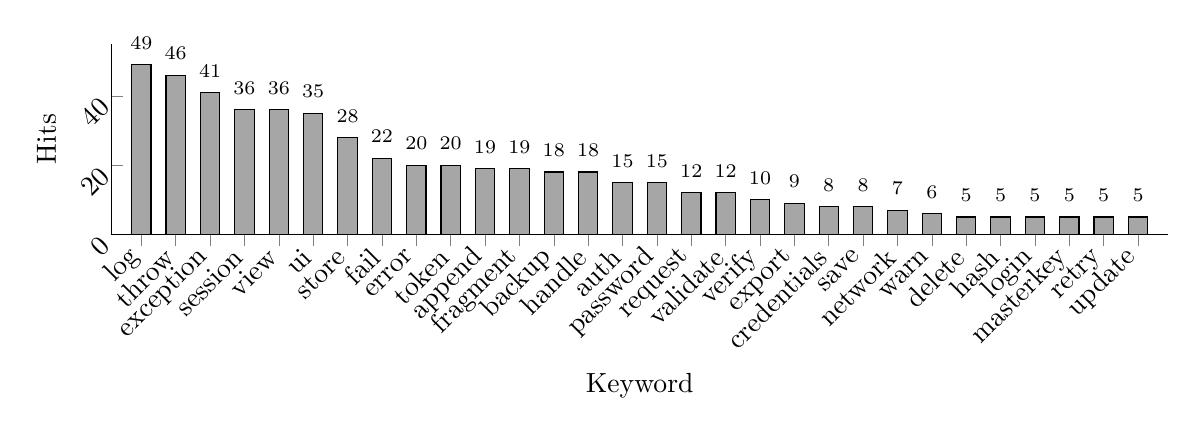
\begin{tikzpicture}
      \begin{axis}[
        width=15cm,
        height=4.0cm,
        ybar,
        bar width=7pt,
        symbolic x coords={
            log,throw,exception,session,view,ui,store,fail,error,token,
            append,fragment,backup,handle,auth,password,request,validate,
            verify,export,credentials,save,network,warn,delete,hash,login,
            masterkey,retry,update},
        xtick=data,
        tick label style={font=\normalsize,rotate=45,anchor=east},
        enlarge x limits=0.03,
        xlabel={Keyword},
        ylabel={Hits},
        ymin=0, ymax=55,
        nodes near coords,
        every node near coord/.append style={font=\scriptsize,yshift=2pt},
        axis x line*=bottom,
        axis y line*=left
      ]
        \addplot[ybar,fill=gray!70] coordinates {
          (log,49) (throw,46) (exception,41) (session,36) (view,36)
          (ui,35) (store,28) (fail,22) (error,20) (token,20) (append,19)
          (fragment,19) (backup,18) (handle,18) (auth,15) (password,15)
          (request,12) (validate,12) (verify,10) (export,9) (credentials,8)
          (save,8) (network,7) (warn,6) (delete,5) (hash,5) (login,5)
          (masterkey,5) (retry,5) (update,5)
        };
      \end{axis}
    \end{tikzpicture}
    \caption{Keyword hits generating categorizations in version diff A. Hits below 5 have been neglected. See Figure \ref{fig:commonly_used_words_A_full} for complete data.}
    \label{fig:commonly_used_words_A}
\end{figure}


\begin{figure}[H]
    \centering
    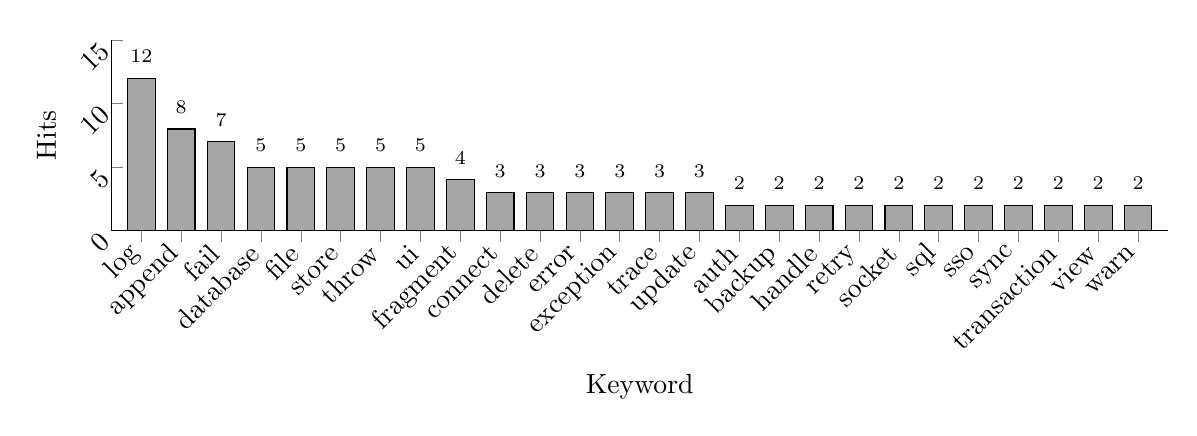
\begin{tikzpicture}
      \begin{axis}[
        width=15cm,
        height=4.0cm,
        ybar,
        bar width=10pt,
        symbolic x coords={
            log,append,fail,database,file,store,throw,ui,fragment,connect,
            delete,error,exception,trace,update,auth,backup,handle,retry,
            socket,sql,sso,sync,transaction,view,warn,commit,credentials,
            debug,decrypt,digest,fetch,hash,refresh,request,send,show,text,
            write},
        xtick=data,
        tick label style={font=\normalsize,rotate=45,anchor=east},
        enlarge x limits=0.03,
        xlabel={Keyword},
        ylabel={Hits},
        ymin=0, ymax=15,
        nodes near coords,
        every node near coord/.append style={font=\scriptsize,yshift=2pt},
        axis x line*=bottom,
        axis y line*=left
      ]
        \addplot[ybar,fill=gray!70] coordinates {
          (log,12) (append,8) (fail,7) (database,5) (file,5) (store,5)
          (throw,5) (ui,5) (fragment,4) (connect,3) (delete,3) (error,3)
          (exception,3) (trace,3) (update,3) (auth,2) (backup,2) (handle,2)
          (retry,2) (socket,2) (sql,2) (sso,2) (sync,2) (transaction,2)
          (view,2) (warn,2)
        };
      \end{axis}
    \end{tikzpicture}
    \caption{Keyword hits generating categorizations in version diff B. Hits below 2 have been neglected. See Figure \ref{fig:commonly_used_words_B_full} for complete data.}
    \label{fig:commonly_used_words_B}
\end{figure}

\begin{figure}[H]
    \centering
    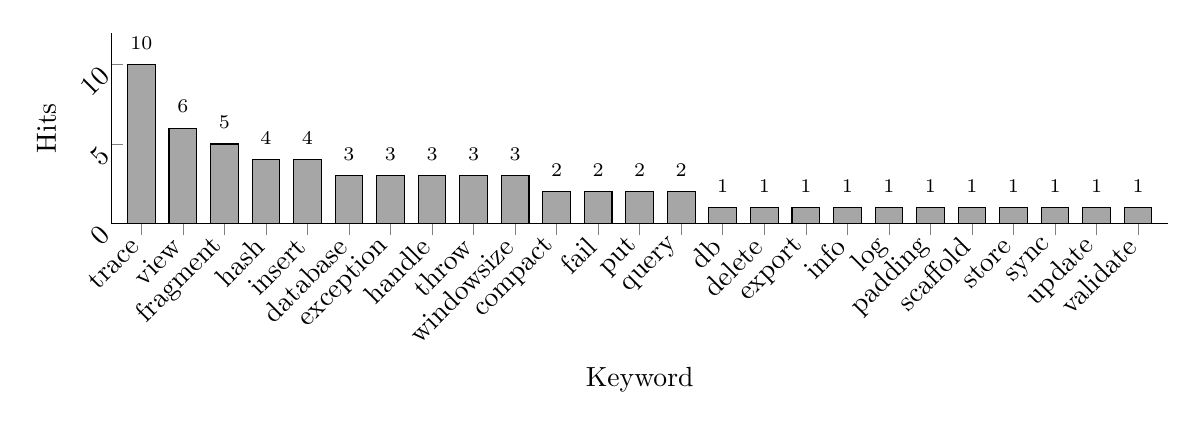
\begin{tikzpicture}
      \begin{axis}[
        width=15cm,
        height=4.0cm,
        ybar,
        bar width=10pt,
        symbolic x coords={
            trace,view,fragment,hash,insert,database,exception,handle,throw,
            windowsize,compact,fail,put,query,db,delete,export,info,log,
            padding,scaffold,store,sync,update,validate},
        xtick=data,
        tick label style={font=\normalsize,rotate=45,anchor=east},
        enlarge x limits=0.03,
        xlabel={Keyword},
        ylabel={Hits},
        ymin=0, ymax=12,
        nodes near coords,
        every node near coord/.append style={font=\scriptsize,yshift=2pt},
        axis x line*=bottom,
        axis y line*=left
      ]
        \addplot[ybar,fill=gray!70] coordinates {
          (trace,10) (view,6) (fragment,5) (hash,4) (insert,4)
          (database,3) (exception,3) (handle,3) (throw,3) (windowsize,3)
          (compact,2) (fail,2) (put,2) (query,2) (db,1) (delete,1)
          (export,1) (info,1) (log,1) (padding,1) (scaffold,1) (store,1)
          (sync,1) (update,1) (validate,1)
        };
      \end{axis}
    \end{tikzpicture}
    \caption{Keyword hits generating categorizations in version diff C (complete)}
    \label{fig:commonly_used_words_C}
\end{figure}



%%%% Commonly used words when incorrect categorization %%%%
\subsubsection{Keywords Resulting in \textit{Incorrect} Categorizations}

This section focuses on the analysis of keywords that resulted in \textit{incorrect} categorizations during the pipeline analysis. Specifically, it examines the total number of times each keyword led to an incorrect classification, providing insights into which keywords are most prone to misclassification.

The results are visualized as bar charts in Figures~\ref{fig:keyword_incorrect_trigger_A}, \ref{fig:keyword_incorrect_trigger_B}, and \ref{fig:keyword_incorrect_trigger_C}. Only keywords that resulted in at least one incorrect categorization are included in these charts. Keywords that did not produce any incorrect hits are excluded to maintain clarity and focus on problematic keywords. This analysis is essential for identifying which keywords may require further refinement or adjustment in the pipeline’s categorization logic to improve overall classification accuracy.


\begin{figure}[H]
    \centering
    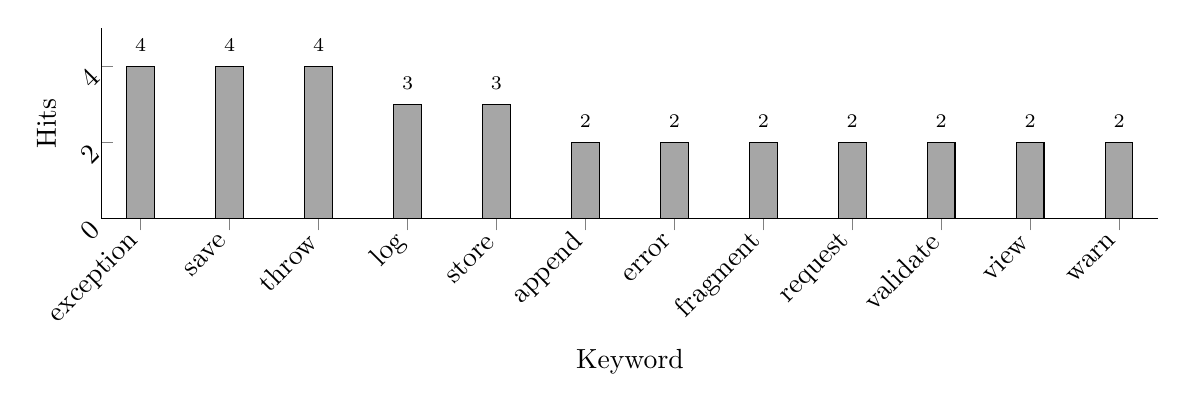
\begin{tikzpicture}
      \begin{axis}[
        width=15cm,
        height=4.0cm,
        ybar,
        bar width=10pt,
        % categorical x-axis
        symbolic x coords={
          exception,save,throw,log,store,append,error,fragment,request,validate,
          view,warn},
        xtick=data,
        tick label style={font=\normalsize,rotate=45,anchor=east},
        enlarge x limits=0.04,
        xlabel={Keyword},
        ylabel={Hits},
        ymin=0, ymax=5,
        nodes near coords,
        every node near coord/.append style={font=\scriptsize,yshift=2pt},
        axis x line*=bottom,
        axis y line*=left
      ]
        \addplot[ybar,fill=gray!70] coordinates {
          (exception,4) (save,4) (throw,4)
          (log,3) (store,3)
          (append,2) (error,2) (fragment,2) (request,2) (validate,2)
          (view,2) (warn,2)
        };
      \end{axis}
    \end{tikzpicture}
    \caption{Keywords resulting in incorrect categorization for version diff A. Hits below 2 have been neglected. See Figure \ref{fig:keyword_incorrect_trigger_A_full} for complete data}
    \label{fig:keyword_incorrect_trigger_A}
\end{figure}

\begin{figure}[H]
    \centering
    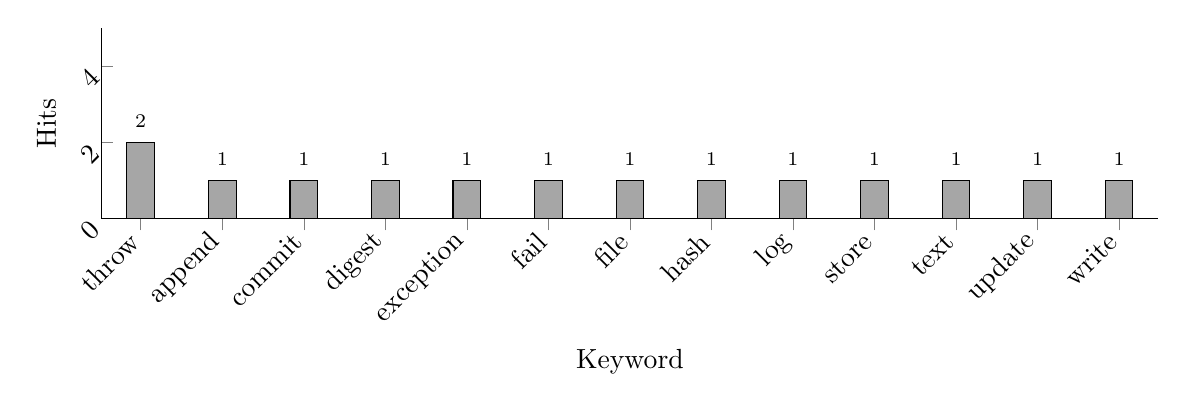
\begin{tikzpicture}
      \begin{axis}[
        width=15cm,
        height=4.0cm,
        ybar,
        bar width=10pt,
        % categorical x-axis
        symbolic x coords={
          throw,append,commit,digest,exception,fail,file,hash,log,store,text,update,write},
        xtick=data,
        tick label style={font=\normalsize,rotate=45,anchor=east},
        enlarge x limits=0.04,
        xlabel={Keyword},
        ylabel={Hits},
        ymin=0, ymax=5,
        nodes near coords,
        every node near coord/.append style={font=\scriptsize,yshift=2pt},
        axis x line*=bottom,
        axis y line*=left
      ]
        \addplot[ybar,fill=gray!70] coordinates {
          (throw,2)
          (append,1) (commit,1) (digest,1) (exception,1) (fail,1)
          (file,1) (hash,1) (log,1) (store,1) (text,1) (update,1) (write,1)
        };
      \end{axis}
    \end{tikzpicture}
    \caption{Keywords resulting in incorrect categorization for version diff B}
    \label{fig:keyword_incorrect_trigger_B}
\end{figure}


\begin{figure}[H]
    \centering
    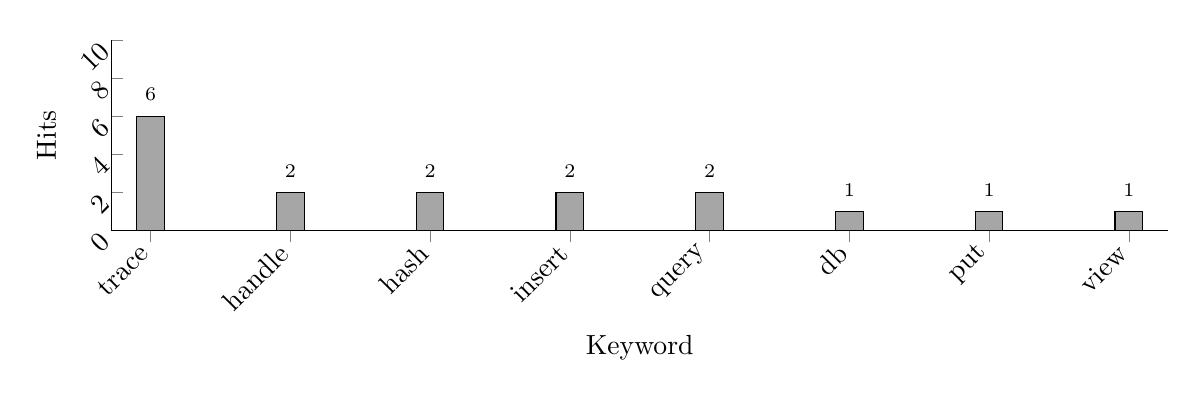
\begin{tikzpicture}
      \begin{axis}[
        width=15cm,
        height=4.0cm,
        ybar,
        bar width=10pt,
        % categorical x-axis
        symbolic x coords={
          trace,handle,hash,insert,query,db,put,view},
        xtick=data,
        tick label style={font=\normalsize,rotate=45,anchor=east},
        enlarge x limits=0.04,
        xlabel={Keyword},
        ylabel={Hits},
        ymin=0, ymax=10,
        nodes near coords,
        every node near coord/.append style={font=\scriptsize,yshift=2pt},
        axis x line*=bottom,
        axis y line*=left
      ]
        \addplot[ybar,fill=gray!70] coordinates {
          (trace,6) (handle,2) (hash,2) (insert,2) (query,2)
          (db,1) (put,1) (view,1)
        };
      \end{axis}
    \end{tikzpicture}
    \caption{Keywords resulting in incorrect categorization for version diff C}
    \label{fig:keyword_incorrect_trigger_C}
\end{figure}




\subsubsection{Accuracy of Keyword Matches}
\label{sec:result:keyword_distribution:Accuracy_of_keyword_matches}

This section examines the accuracy of keyword-based categorizations in the pipeline analysis, focusing on how effectively each keyword triggers correct classifications. The accuracy of keyword matches is visualized in three separate figures—Figures~\ref{fig:keyword_match_accuracy_A}, \ref{fig:keyword_match_accuracy_B}, and \ref{fig:keyword_match_accuracy_C}—each corresponding to one of the three analyzed version differences (A, B, and C). These figures provide a clear view of the performance of each keyword in accurately categorizing changes. Keywords with matches below 2 have been
neglected from the figures.

Recall that a match is deemed correct when the pipeline assigns any category that also appears in the manual review; if none of its categories overlap, the match is incorrect—even when the pipeline captures parts of the manual set. See Section \ref{sec:result:understanding_correct_incorrect} for full definition. This approach may result in an inflated count of \textit{correct} matches, as keywords are credited with success whenever there is any overlap with the manually identified categories. Similarly, the number of \textit{incorrect} matches may be slightly deflated, as partially correct categorizations are also marked as incorrect. This distinction is crucial for accurately interpreting the results shown in the figures.



\begin{figure}[H]
  \centering
    \begin{tikzpicture}
    \begin{axis}[%
      xbar stacked,
      width=13.5cm,height=22cm,
      bar width=8pt,
      symbolic y coords={
        log,throw,exception,session,ui,view,store,fail,token,backup,error,append,
        fragment,handle,auth,password,request,validate,verify,export,credentials,
        network,hash,login,update,delete,masterkey,retry,save,warn,database,
        debug,info,file,insert,query,show,sync,text},
      ytick=data,
      tick label style={font=\small},
      xmin=0,xmax=100,
      xtick={0,20,...,100},
      xlabel={Accuracy},
      ylabel={Keyword},
      nodes near coords={\pgfmathprintnumber[fixed,precision=2]{\pgfplotspointmeta}\%},
      enlarge y limits=0.02,
      legend style={at={(0.5,-0.05)},anchor=north,legend columns=-1},
    ]
      % ─── Correct (green) ────────────────────────────
      \addplot[fill=correct_color] coordinates {
        (93.88,log) (91.30,throw) (90.24,exception) (97.22,session)
        (97.14,ui) (94.44,view) (89.29,store) (100.00,fail)
        (95.00,token) (100.00,backup) (90.00,error) (89.47,append)
        (89.47,fragment) (94.44,handle) (93.33,auth) (93.33,password)
        (83.33,request) (83.33,validate) (100.00,verify) (100.00,export)
        (100.00,credentials) (85.71,network) (100.00,hash) (100.00,login)
        (100.00,update) (80.00,delete) (80.00,masterkey) (80.00,retry)
        (50.00,save) (66.67,warn) (75.00,database) (100.00,debug)
        (75.00,info) (66.67,file) (66.67,insert) (100.00,query)
        (100.00,show) (100.00,sync) (100.00,text)};
      % ─── Incorrect (red) ────────────────────────────
      \addplot[fill=incorrect_color] coordinates {
        ( 6.12,log) ( 8.70,throw) ( 9.76,exception) ( 2.78,session)
        ( 2.86,ui)  ( 5.56,view)  (10.71,store)  ( 0.00,fail)
        ( 5.00,token)( 0.00,backup)(10.00,error) (10.53,append)
        (10.53,fragment)( 5.56,handle)( 6.67,auth) ( 6.67,password)
        (16.67,request)(16.67,validate)( 0.00,verify)( 0.00,export)
        ( 0.00,credentials)(14.29,network)( 0.00,hash)( 0.00,login)
        ( 0.00,update)(20.00,delete)(20.00,masterkey)(20.00,retry)
        (50.00,save) (33.33,warn) (25.00,database)( 0.00,debug)
        (25.00,info) (33.33,file) (33.33,insert)( 0.00,query)
        ( 0.00,show) ( 0.00,sync) ( 0.00,text)};
      \legend{Correct,Incorrect}
    \end{axis}
  \end{tikzpicture}
  \caption{Keyword match accuracy, for version diff A}
  \label{fig:keyword_match_accuracy_A}
\end{figure}



\begin{figure}[H]
  \centering
    \begin{tikzpicture}
    \begin{axis}[%
      xbar stacked,
      width=13.5cm,height=14cm,
      bar width=8pt,
      symbolic y coords={
        log,append,fail,database,ui,file,fragment,store,connect,delete,error,
        throw,trace,auth,backup,exception,handle,retry,socket,sql,sso,sync,
        transaction,update,view,warn},
      ytick=data,
      tick label style={font=\small},
      xmin=0,xmax=100,
      xtick={0,20,...,100},
      xlabel={Accuracy},
      ylabel={Keyword},
      nodes near coords={\pgfmathprintnumber[fixed,precision=2]{\pgfplotspointmeta}\%},
      enlarge y limits=0.02,
      legend style={at={(0.5,-0.1)},anchor=north,legend columns=-1},
    ]
      % ─── Correct (green) ────────────────────────────
      \addplot[fill=correct_color] coordinates {
        (91.67,log) (87.50,append) (85.71,fail) (100.00,database)
        (100.00,ui) (80.00,file) (100.00,fragment) (80.00,store)
        (100.00,connect) (100.00,delete) (100.00,error) (60.00,throw)
        (100.00,trace) (100.00,auth) (100.00,backup) (66.67,exception)
        (100.00,handle) (100.00,retry) (100.00,socket) (100.00,sql)
        (100.00,sso) (100.00,sync) (100.00,transaction) (66.67,update)
        (100.00,view) (100.00,warn)};
      % ─── Incorrect (red) ────────────────────────────
      \addplot[fill=incorrect_color] coordinates {
         (8.33,log) (12.50,append) (14.29,fail) ( 0.00,database)
         ( 0.00,ui)  (20.00,file)  ( 0.00,fragment) (20.00,store)
         ( 0.00,connect) ( 0.00,delete) ( 0.00,error) (40.00,throw)
         ( 0.00,trace) ( 0.00,auth) ( 0.00,backup) (33.33,exception)
         ( 0.00,handle) ( 0.00,retry) ( 0.00,socket) ( 0.00,sql)
         ( 0.00,sso) ( 0.00,sync) ( 0.00,transaction) (33.33,update)
         ( 0.00,view) ( 0.00,warn)};
      \legend{Correct,Incorrect}
    \end{axis}
  \end{tikzpicture}
  \caption{Keyword match accuracy, for version diff B}
  \label{fig:keyword_match_accuracy_B}
\end{figure}


\begin{figure}[H]
  \centering
    \begin{tikzpicture}
    \begin{axis}[%
      xbar stacked,
      width=13.5cm,height=14cm,
      bar width=8pt,
      symbolic y coords={
        fragment,view,trace,database,exception,throw,windowsize,compact,fail,
        hash,insert,delete,export,handle,info,log,padding,put,scaffold,store,
        sync,update,validate},
      ytick=data,
      tick label style={font=\small},
      xmin=0,xmax=100,
      xtick={0,20,...,100},
      xlabel={Accuracy},
      ylabel={Keyword},
      nodes near coords={\pgfmathprintnumber[fixed,precision=2]{\pgfplotspointmeta}\%},
      enlarge y limits=0.02,
      legend style={at={(0.5,-0.1)},anchor=north,legend columns=-1},
    ]
      % ─── Correct (green) ────────────────────────────
      \addplot[fill=correct_color] coordinates {
        (100.00,fragment) (83.33,view) (40.00,trace) (100.00,database)
        (100.00,exception) (100.00,throw) (100.00,windowsize) (100.00,compact)
        (100.00,fail) (50.00,hash) (50.00,insert) (100.00,delete) (100.00,export)
        (33.33,handle) (100.00,info) (100.00,log) (100.00,padding) (50.00,put)
        (100.00,scaffold) (100.00,store) (100.00,sync) (100.00,update)
        (100.00,validate)};
      % ─── Incorrect (red) ────────────────────────────
      \addplot[fill=incorrect_color] coordinates {
         ( 0.00,fragment) (16.67,view) (60.00,trace) ( 0.00,database)
         ( 0.00,exception) ( 0.00,throw) ( 0.00,windowsize) ( 0.00,compact)
         ( 0.00,fail) (50.00,hash) (50.00,insert) ( 0.00,delete) ( 0.00,export)
         (66.67,handle) ( 0.00,info) ( 0.00,log) ( 0.00,padding) (50.00,put)
         ( 0.00,scaffold) ( 0.00,store) ( 0.00,sync) ( 0.00,update)
         ( 0.00,validate)};
      \legend{Correct,Incorrect}
    \end{axis}
  \end{tikzpicture}
  \caption{Keyword match accuracy, for version diff C}
  \label{fig:keyword_match_accuracy_C}
\end{figure}





%%%%%%%%%%%%%%%%%%%%%%%%%%%%%%
% COMBINED TOTAL RESULT
%%%%%%%%%%%%%%%%%%%%%%%%%%%%%%
\subsection{Comprehensive summary of version diffs}
\label{sec:res:comprehensive_summary}

\subsubsection{Summarized pipeline accuracy}
The table in Figure~\ref{tab:overall_accuracy} presents a comprehensive overview of the pipeline's accuracy, aggregated across all three version differences (diffs). This table provides a summary of the pipeline’s performance in three key aspects:

\begin{itemize}
    \item \textbf{Change Detection Accuracy:} This metric indicates how effectively the pipeline detects changes between the analyzed versions. It is calculated as the proportion of changes identified by the pipeline compared to the total changes identified during the manual analysis.

    \item \textbf{Status Accuracy:} This metric measures the pipeline's ability to correctly determine the status of each detected change—whether it is an addition, modification, or deletion. It reflects how well the pipeline aligns with the manual analysis in classifying the type of each change.

    \item \textbf{Categorization Accuracy:} This metric assesses how accurately the pipeline assigns categories to the detected changes. It is calculated by comparing the categories assigned by the pipeline with those identified during the manual analysis. A correct categorization is counted when the pipeline's assigned categories match or overlap with those determined manually.

\end{itemize}

By aggregating the accuracy results across all three version diffs, this table provides a holistic view of the pipeline’s overall performance. It helps identify strengths and weaknesses in the change detection, status classification, and categorization processes, offering valuable insights for further improvement.


\begin{comment}
FOUND ACCURACY = (81+21+26)/(84+28+28) = 0,9142857143
STATUS ACCURACY = (71+16+23)/(84+28+28) = 0,7857142857

TOT CATEGORY ACCURACY = (72+17+15)/(84+28+28) = 0,7428571429
CATEGORY ACCURACY CRITICAL = (48+9+3)/(57+16+4) = 0,7792207792
CATEGORY ACCURACY NON-CRIT = (24+8+12)/(27+12+24) = 0,6984126984
\end{comment}

\begin{table}[H]
    \centering
    \begin{tabular}{l l}
        \toprule
        \textbf{Metric} & \textbf{Accuracy} \\
        \midrule
        Changes detected & 91.4\% \\
        Correct change status & 78.6\% \\
        Correctly set categories & 74.3\% \\
        \textit{\ \ \ \ \ \ \ \ Critical categories} & 77.9\% \\
        \textit{\ \ \ \ \ \ \ \ Non-critical categories} & 69.8\% \\
        \bottomrule
    \end{tabular}
    \caption{Combined pipeline accuracy metrics.}
    \label{tab:overall_accuracy}
\end{table}


\subsubsection{Summarized Category Assignment Accuracy}

As previously mentioned in Section~\ref{sec:result:categorization_distributions:categories_resulting_in_correct_incorrect_categorizations}, the categories \codebox{UI update} and \codebox{Authentication} demonstrated the highest accuracy in correct category assignments. This observation is further supported by the detailed accuracy analysis presented in Figures~\ref{fig:correct_incorrect_categorization_accuracy_critical} and \ref{fig:correct_incorrect_categorization_accuracy_noncritical}, which provide a clear view of the correct and incorrect categorization rates for each category.

A closer look at these figures reveals that some categories, such as \codebox{File write}, \codebox{Cryptographic}, and \codebox{Text manipulation}, exhibit 0\% accuracy in correct assignments. However, this result is misleading because the total number of assignments for these categories is either extremely low or nonexistent. Consequently, even a single incorrect categorization can significantly skew the accuracy percentage for these categories.

Additionally, the category \codebox{Error handling} shows consistently low accuracy, even though it has a substantial number of assignments, both correct and incorrect. This suggests that the categorization keywords associated with \codebox{Error handling} may require refinement to improve accuracy.

From these observations, it is clear that the critical categories \codebox{Authentication} and \codebox{Data storage}, along with the non-critical categories \codebox{UI update} and \codebox{Network call}, have keyword definitions that are highly effective in producing accurate and reliable categorizations. These categories benefit from well-defined and contextually relevant keywords, leading to consistent and correct classifications. High accuracy of the non-critical categories like \codebox{UI update} and \codebox{Network call} is beneficial when analyzing the tool's report. Accurately filtering out unimportant changes reduces the number of critical changes to investigate, making the manual review process more focused and efficient.


\begin{table}[H]
    \centering

    \begin{tikzpicture}
        \begin{axis}[%
        xbar stacked,
        width=10cm,height=6cm,
        bar width=15pt,
        %
        % ── value labels ────────────────────────────────
        nodes near coords={\pgfmathprintnumber[fixed,precision=2]{\pgfplotspointmeta}\%},
        %
        xmin=0,xmax=100,
        xtick={0,10,...,100},
        ytick={1,...,6},
        yticklabels={
          Cryptographic,
          File write,
          Error handling,
          Logging,
          Data storage,
          Authentication},
        xtick pos=bottom,
        ytick pos=left,
        xticklabel={\pgfmathprintnumber[fixed,precision=2]{\tick}\%},
        enlarge y limits=.15,
        legend style={at={(0.5,-0.20)},anchor=north,legend columns=-1},
        ]
        % ─── Correct (green) ────────────────────────────
        \addplot[xbar,fill=correct_color] coordinates {
          (0,1) (0,2) (22.22,3) (53.85,4) (70.37,5) (91.43,6)};
        % ─── Incorrect (red) ────────────────────────────
        \addplot[xbar,fill=incorrect_color] coordinates {
          (100,1) (100,2) (77.78,3) (46.15,4) (29.63,5) (8.57,6)};
        \legend{Correct,Incorrect}
        \end{axis}
    \end{tikzpicture}
    
    \caption{Total ratio of correct vs incorrect assignment of critical categories.}
    \label{fig:correct_incorrect_categorization_accuracy_critical}
\end{table}


\begin{table}[H]
    \centering

    \begin{tikzpicture}
        \begin{axis}[%
        xbar stacked,
        width=10cm,height=4cm,
        bar width=15pt,
        %
        % ── value labels ────────────────────────────────
        nodes near coords={\pgfmathprintnumber[fixed,precision=2]{\pgfplotspointmeta}\%},
        %
        xmin=0,xmax=100,
        xtick={0,10,...,100},
        ytick={1,...,3},
        yticklabels={
          Text manipulation,
          Network call,
          UI update},
        xtick pos=bottom,
        ytick pos=left,
        xticklabel={\pgfmathprintnumber[fixed,precision=2]{\tick}\%},
        enlarge y limits=0.35,
        legend style={at={(0.5,-0.20)},anchor=north,legend columns=-1},
        ]
        % ─── Correct (green) ────────────────────────────
        \addplot[xbar,fill=correct_color] coordinates {
          (0,1) (83.33,2) (92.86,3)};
        % ─── Incorrect (red) ────────────────────────────
        \addplot[xbar,fill=incorrect_color] coordinates {
          (100,1) (16.67,2) (7.14,3)};
        \legend{Correct,Incorrect}
        \end{axis}
    \end{tikzpicture}
    
    \caption{Total ratio of correct vs incorrect assignment of non-critical categories.}
    \label{fig:correct_incorrect_categorization_accuracy_noncritical}
\end{table}
